% vim:set et fenc=utf-8 ft=tex sw=2 ts=2 tw=72:

\newif\ifdraft
\drafttrue

\ifdraft
        \documentclass[draft]{IEEEtran}
        \def\baselinestretch{1}
        % \setlength{\marginparwidth}{1.5cm}
\else
        \documentclass[conference]{IEEEtran}
\fi

% vim:set et sw=2 ts=4 tw=72:
\usepackage[T1]{fontenc}
\usepackage[utf8]{inputenc}
\usepackage[hyphens]{url}
\urlstyle{same}

%% Citations
\usepackage[nospace]{cite}

%% Table Support
\usepackage{array}
\usepackage{dcolumn}
\usepackage{longtable}
\usepackage{multirow}
\usepackage{booktabs}
\usepackage{tabulary}

%% Extra support
\usepackage{xspace}
\usepackage{amsmath}
\usepackage{amssymb}
\usepackage{balance}
\usepackage{placeins}
\usepackage{fancyvrb}

%% Algorithms
\usepackage{algorithm}
\usepackage{algpseudocode}

%% Graphics
\usepackage{tikz}
\usepackage{pgfplots}
\usepackage{pgfplotstable}
\usepackage{xcolor}
\usepackage{color}
\usepackage{listings}


\usetikzlibrary{positioning, arrows}

% Chart Colors
\definecolor{chartblue}{HTML}{3366CC}
\definecolor{chartred}{HTML}{DC3912}
\definecolor{chartyellow}{HTML}{FF9900}
\definecolor{chartgreen}{HTML}{109618}
\definecolor{chartmagenta}{HTML}{990099}
\definecolor{chartpurple}{HTML}{3B3EAC}

% \ifdraft
%     \usepackage[colorinlistoftodos]{todonotes}
%     \newcommand{\evan}[1]{{\color{blue}\emph{Evan Says: #1}}\xspace}
%     \newcommand{\evantodo}[1]{{\color{blue}\emph{Evan Todo: #1}}\xspace}
%     \newcommand{\dmg}[1]{{\color{blue}\emph{dmg Says: #1}}\xspace}
%     \newcommand{\dmgtodo}[1]{{\color{blue}\emph{dmg Todo: #1}}\xspace}
% \else
%     \usepackage[disable]{todonotes}
%     \newcommand{\evan}[1]{}
%     \newcommand{\evantodo}[1]{}
%     \newcommand{\dmg}[1]{}
%     \newcommand{\dmgtodo}[1]{}
% \fi
    \usepackage[colorinlistoftodos]{todonotes}

\newcommand{\tool}{{\emph Linvis}\xspace}


    \newcommand{\evan}[1]{{\color{blue}\emph{Evan Says: #1}}\xspace}
    \newcommand{\evantodo}[1]{{\color{blue}\emph{Evan Todo: #1}}\xspace}
    \newcommand{\dmg}[1]{{\color{blue}\emph{dmg Says: #1}}\xspace}
    \newcommand{\dmgtodo}[1]{{\color{blue}\emph{dmg Todo: #1}}\xspace}


%%% Local Variables:
%%% mode: plain-tex
%%% TeX-master: t
%%% End:


\newcommand{\TheTitle}{Merge-Tree: Visualizing the Integration of Commits into Linux}
\newcommand{\TheAuthors}{Evan Wilde, Daniel M. German}
\newcommand{\TheEmails}{etcwilde@uvic.ca, dmg@uvic.ca}
\newcommand{\TheSubject}{Understanding a large number of commits and merges}
\newcommand{\TheKeywords}{Linux, git, visualizations, Merge-Tree}

%% Referencing
\usepackage[unicode=true,
          pdftitle={\TheTitle},
          pdfauthor={\TheAuthors},
          colorlinks=false]{hyperref}


\algdef{SE}[DOWHILE]{Do}{doWhile}{\algorithmicdo}[1]{\algorithmicwhile\ #1}%

\lstset{frame=tb,
  language=python,
  aboveskip=3mm,
  belowskip=3mm,
  showstringspaces=false,
  columns=flexible,
  basicstyle={\small\ttfamily},
  numbers=none,
  numberstyle=\tiny\color{gray},
  keywordstyle=\color{chartblue},
  commentstyle=\color{chartred},
  stringstyle=\color{chartgreen},
  breaklines=true,
  breakatwhitespace=true,
  tabsize=3
}

\synctex=1

\hyphenation{Correctness Accuracy Timing Commit}



\begin{document}

\title{\TheTitle}

\author{
        \IEEEauthorblockA{\TheAuthors}
        \IEEEauthorblockN{Department of Computer Science,
                University of Victoria, Canada.}
        \IEEEauthorblockA{Email: \TheEmails}
}
\maketitle

\begin{abstract}

  % vim:set et sw=2 ts=4 tw=72:
With an average of more than 900 top-level merges into the Linux kernel
per release, many containing hundreds of commits and some containing
thousands, maintenance of older versions of the kernel becomes nearly
impossible.  Various commercial products, such as the Android platform,
run older versions of the kernel. Due to security, performance, and
changing hardware needs, maintainers must understand what changes
(commits) are added to the current version of the kernel since the last
time they inspected it in order to make the necessary patches.

Current tools provide information about repositories through the
directed acyclic graph (DAG) of the repository, which is helpful for
smaller projects. However, with the scale and number of branches in the
kernel the DAG becomes overwhelming very quickly. Furthermore, the DAG
contains every ancestor of every commit, while maintainers are more
interested in how and when a commit arrives to the official Linux
repository.

In this paper, we propose the merge-tree, a simplified transformation of
the DAG of the Linux git repository that shows the way in which commits
are merged into the master branch of Linux. Using the merge-tree, we
build \tool, a tool that is designed to allow users to explore how
commits are merged into the Linux kernel.

\dmg{add to the abstract the user study}

%%% Local Variables:
%%% mode: latex
%%% TeX-master: "lineval.tex"
%%% End:


\end{abstract}


\begin{IEEEkeywords}
  \TheKeywords
\end{IEEEkeywords}

\section{Introduction}

% vim:set et sts=2 sw=2 ts=2 tw=72:

Between 50k and 70k commits are added to the Linux kernel per version,
requiring maintainers of older versions of the kernel to sift through
thousands of commits and merges with tools that are unable to filter and
effectively visualize projects at the scale of the kernel. Older
versions of the kernel are used in embedded systems and mobile phones;
for security purposes, performance needs, and changing hardware
requirements, maintainers must be able to understand the changes being
made in the current version of the kernel in order to produce the
necessary patches for the older versions of the kernel. Tools like Gitk
use a directed acyclic graph (DAG) model of the repository, showing all
commits and merges in chronological order by when the commit was
authored, not by when it arrived in the official Linux repository.

\begin{figure}
        \centering
        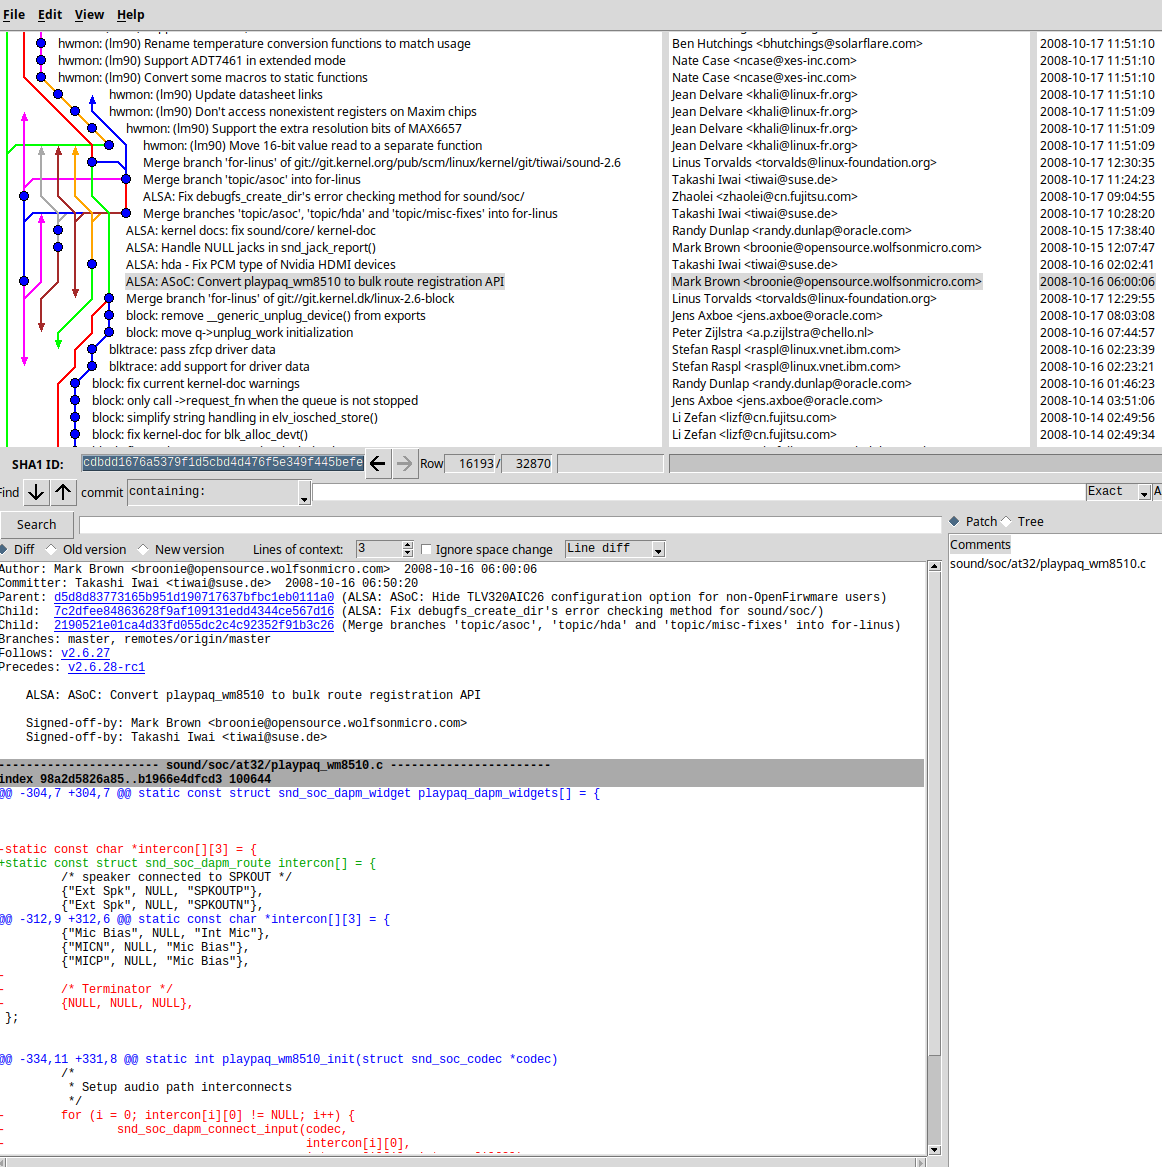
\includegraphics[width=0.97\linewidth]{figures/gitk.png}
        \caption{The Gitk interface centered on commit
          cdbdd1676a5379f1d5cbd4d476f5e349f445befe, \comB from the user
          study. The top-left pane shows the DAG and commit log preview,
          the top center pane shows the authors, and the top-right
          pane shows the commit dates. The bottom-left pane shows the
          full commit message, the parents and children of the commit,
          and the changes made to files in this commit. The bottom-right
          pane shows the list of the files modified by this commit.}
        \label{fig:gitk}
%\vspace{-4mm}
\end{figure}

\begin{figure}
        \centering
        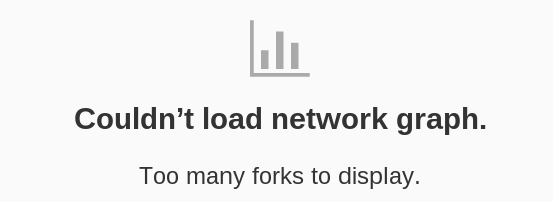
\includegraphics[width=0.8\linewidth]{figures/github_viewer.png}
        \caption{Github normally shows a visualization of the DAG,
          showing the commits, branches, and forks, but is unable to
          generate a visualization for projects at the size of the Linux
          repository.}
        \label{fig:gitfail}
%\vspace{-2mm}
\end{figure}

The DAG is able to provide a meaningful visualization in smaller
projects; it enables users to see when changes are made, when these
changes are merged, how each branch is interacting, and the point where
a branch forks from the master branch. In large modular projects, like
the Linux kernel, the DAG becomes a mess of merges and commits
(Figure~\ref{fig:gitk}) losing its visual meaning. In some cases, the
Linux kernel is simply too large for the system to generate a
visualization; Github provides a DAG view for many projects, but is
unable to display the visualization for projects at the scale of the
Linux of the kernel (Figure~\ref{fig:gitfail}). Between 60k and 70k new
commits are created for the Linux project every year; according to
previous work\cite{German2015}, a commit takes a median of 30 days from
the time it is authored until it arrives in the official repository. The
snapshot of the kernel tomorrow may be different than the snapshot from
today, containing new commits authored in the past; distinguishing these
new commits from the commits in the snapshot from today is not trivial.

One major challenge with visualizing the arrival of commits to a
repository is that Git does not store the date that a commit was merged
into another branch, including the master branch. To complicate the
problem, the DAG only has references to the ancestors of a commit (a
model necessary for the operation of Git), but maintainers would prefer
knowing the path a commit followed to reach the master repository.
Tracing a path that any commit followed to the master repository would
imply that for any given merge, it would be possible to know which
commits were merged. A user could inspect the commits that arrived into
the master branch within a given time-frame by checking which commits
were merged during that time-frame.

This paper makes three contributions; first, we describe a method of
converting the DAG of the Linux repository into the \mt of the
repository, that represents the path used by a commit to reach the
master branch; second, we present an implementation enabling the
inspection and visualization of merges in the Linux project using the
\mt modle; finally, we validate the \mt model and the implementation of
the visulization through a controlled user study. We further discuss the
issues of generalizing the model to other repositories, but present an
updated version that improves the performance of the algorithm by
pruning the DAG.\@

These methods and visualizations are implemented in a web-based tool
called \tool\footnote{\tool is currently available at
  \url{http://li.turingmachine.org}}. Our visualizations and tool
provide information about the location of any given commit or merge in
its respective merge-tree, the files edited, the modules edited, and the
commit message. \tool allows users to apply various filters, including
the release version, along with a keyword or phrase from the log
preview, the name of the author, or the commit hash. The user can
request all merges made by Linus that contain a commit or inner merge
that matches the search query, or just the commits and merges that match
the query.


\section{Merge-Tree model}
\label{sec:mergetree}

% vim:set et sw=2 ts=4 tw=72:

\section{Merge-Tree model}
\label{sec:mergetree}

The \mt model abstracts the DAG of the repository into a set of \mt{s}.
Each \mt is rooted at a merge into the master branch. The leaves of this
tree are the commits and the merges are the inner nodes. A \mt is built
recursively with every merge in the \mt merging a sub-\mt. Any merges
that a commit must pass through to reach the master branch become an
inner node of the tree. Effectively, a \mt is a tree that shows the path
that commits follow in their way to the master branch of a repository.
The \mt{s} also help understand how commits were grouped together in
order to be integrated. In this model, not only has the DAG been
inverted (and simplified), but the entire notion of parent-child
relationship has been reversed. Due to this property, the terminology
will be different depending on the model we are referring to; when we
are referring to the \mt, the parent is the next node toward the merge
into the master branch, or the root of the tree. When referring to the
DAG, the parent relationship is in the opposite direction, from the root
toward the branch-point. In addition to identifying the path that a
commit took to being merged, we are able to aggregate the commit
metadata at merges as we retain the parent-child and child-parent
relationship for each event and know which commits belong to the merge.

To illustrate this model we will use a small example: assume the commits
represented in Figure~\ref{fig:repoEvents} show the sequence of events
in a repository. The sequence starts with the initial commit in the
master branch of the master repository at time $t_0$. Repository event 1
is a commit, which gets forked into a separate repository, \textit{Repo
  A}, where another commit is made, event 2. Event 5 is a merge event,
merging event 2, 3, and 4 into \textit{Repo A}. Event 5 is branched
from, commit 6 happens in the new branch, while commit 7 is added
simultaneously to the original branch in \textit{Repo A}. Events 11 and
12 are both merge events, merging changes made in \textit{Repo A} into
the master branch of the master repository. As every repository is a
first-class repository, including local copies and forks, git does not
distinguish between forked repositories and branches, and in neither
case does it explicitly record where a commit was made. In this case,
commits are performed in various repositories and branches. The DAG
representation of these events is shown in Figure~\ref{fig:repoDAG}.

Notice that the DAG loses information about the master branch and the
repository that the master branch is part of. The \mt view of
this DAG is visible in Figure~\ref{fig:repoTree}. Note that the
direction of the edges of the DAG have been inverted, instead of
pointing from the child to the parent, it points from the parent to its
children, forming a path to the master branch. Also note that the DAG
has been simplified, showing only a single edge on the path to master
for any commit.

\begin{figure}[htbp]
  \centering
  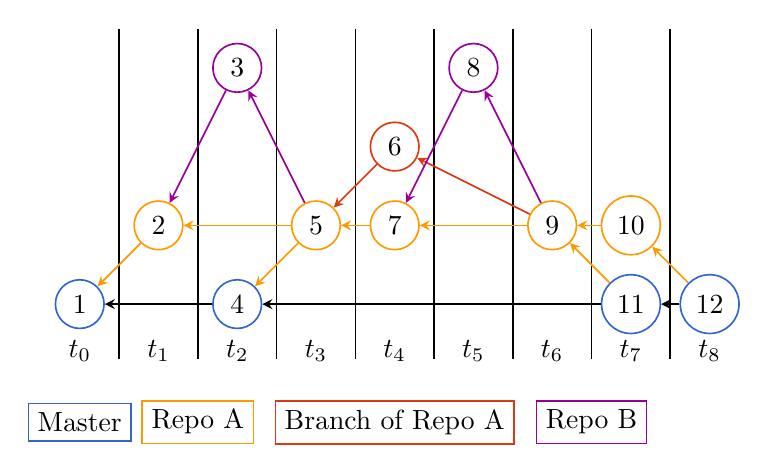
\begin{tikzpicture}[auto, on grid, semithick, state/.style={circle, text=black}]
    \foreach \x in {0, 1, 2, 3, 4, 5, 6, 7}
    \draw[shift={(\x + 0.5, -0.5)}, color=black] (0cm, 4cm) -- (0pt, -0.2cm);

    \node[state, draw=chartblue] (1) {1};
    \node[state, draw=chartyellow, above right= of 1] (2) {2};
    \node[state, draw=chartmagenta, above right= 2cm and 1cm of 2] (3) {3};
    \node[state, draw=chartblue, right= 2cm of 1] (4) {4};
    \node[state, draw=chartyellow, above right=of 4] (5) {5};
    \node[state, draw=chartred, above right=of 5] (6) {6};
    \node[state, draw=chartyellow, right=of 5] (7) {7};
    \node[state, draw=chartmagenta, above right= 2cm and 1cm of 7](8) {8};
    \node[state, draw=chartyellow, right= 2cm of 7] (9) {9};
    \node[state, draw=chartyellow, right=of 9] (10) {10};
    \node[state, draw=chartblue, below right=of 9] (11) {11};
    \node[state, draw=chartblue, below right=of 10] (12) {12};

    \draw (12) edge[-stealth] (11) edge[chartyellow, -stealth] (10);
    \draw (11) edge[-stealth] (4) edge[chartyellow, -stealth] (9);
    \draw (10) edge[chartyellow, -stealth] (9);
    \draw (9) edge[chartmagenta, -stealth] (8) edge[chartred, -stealth] (6)
              edge[chartyellow, -stealth] (7);
    \draw (8) edge[chartmagenta, -stealth] (7);
    \draw (7) edge[chartyellow, -stealth] (5);
    \draw (6) edge[chartred, -stealth] (5);
    \draw (5) edge[chartmagenta, -stealth] (3) edge[chartyellow,-stealth] (2)
              edge[chartyellow, -stealth] (4);
    \draw (4) edge[-stealth] (1);
    \draw (3) edge[chartmagenta, -stealth] (2);
    \draw (2) edge[chartyellow, -stealth] (1);

    \node [draw=chartblue, below = 1.5cm of 1] (l1) {Master};
    \node [draw=chartyellow, right = 1.5cm of l1] (l2) {Repo A};
    \node [draw=chartred, right = 2.5cm of l2] (l3) {Branch of Repo A};
    \node [draw=chartmagenta, right= 2.5cm of l3] (l4) {Repo B};

        \foreach \x in {0, 1, 2, 3, 4, 5, 6, 7, 8}
    \node[shift={(\x, -0.6)}, color=black] {$t_\x$};
  \end{tikzpicture}
  \caption{Example of a sequence of events performed in different
    repositories. The horizontal axis represents time. Each horizontal
    section represents a different branch and/or repository. Each commit
    points to its parent. The intial commit is at time $t_0$, and the
    head is at $t_8$.}
  \label{fig:repoEvents}
%\vspace{-3mm}
\end{figure}

\begin{figure}[htbp]
  \centering
  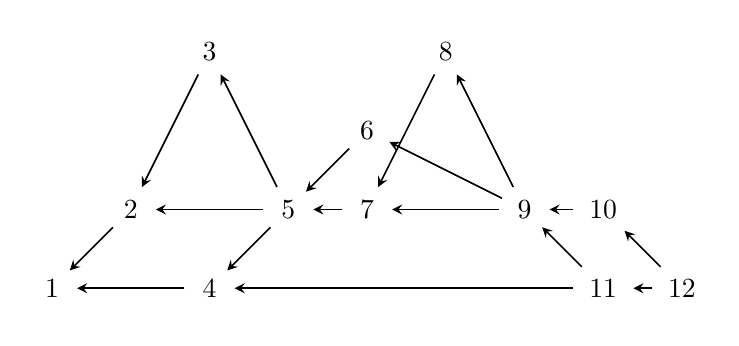
\begin{tikzpicture}[auto, on grid, semithick, state/.style={circle, text=black, black}]
    \node[state, black] (1) {1};
    \node[state, black, above right= of 1] (2) {2};
    \node[state, black, above right= 2cm and 1cm of 2] (3) {3};
    \node[state, black, right= 2cm of 1] (4) {4};
    \node[state, black, above right=of 4] (5) {5};
    \node[state, black, above right=of 5] (6) {6};
    \node[state, black, right=of 5] (7) {7};
    \node[state, black, above right= 2cm and 1cm of 7](8) {8};
    \node[state, black, right= 2cm of 7] (9) {9};
    \node[state, black, right=of 9] (10) {10};
    \node[state, black, below right=of 9] (11) {11};
    \node[state, black, below right=of 10] (12) {12};

    \draw (12) edge[-stealth] (11) edge[-stealth] (10);
    \draw (11) edge[-stealth] (4) edge[-stealth] (9);
    \draw (10) edge[-stealth] (9);
    \draw (9) edge[-stealth] (8) edge[-stealth] (6)
              edge[-stealth] (7);
    \draw (8) edge[-stealth] (7);
    \draw (7) edge[-stealth] (5);
    \draw (6) edge[-stealth] (5);
    \draw (5) edge[-stealth] (3) edge[-stealth] (2)
              edge[-stealth] (4);
    \draw (4) edge[-stealth] (1);
    \draw (3) edge[-stealth] (2);
    \draw (2) edge[-stealth] (1);
  \end{tikzpicture}
  \caption{DAG representation of the commits represented in
    Figure~\ref{fig:repoEvents}. The DAG loses information about which
    repository the commit is performed in and through which merges it
    has passed on its way to the master branch. The DAG does not even
    distinguish the master branch from other branches.}
  \label{fig:repoDAG}
%\vspace{-3mm}
\end{figure}

\begin{figure}[htbp]
  \centering
  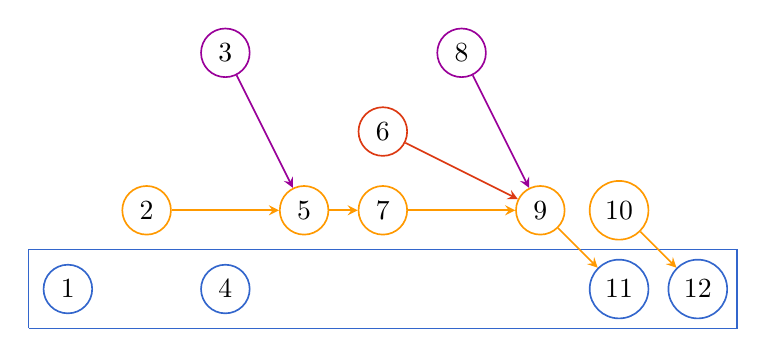
\begin{tikzpicture}[auto, on grid, semithick, state/.style={circle, text=black}]

    \draw[chartblue]
      (-0.5, -0.5) -- (8.5, -0.5) -- (8.5, 0.5) -- (-0.5, 0.5) -- (-0.5, -0.5);

    \node[state, draw=chartblue] (1) {1};
    \node[state, draw=chartyellow, above right= of 1] (2) {2};
    \node[state, draw=chartmagenta, above right= 2cm and 1cm of 2] (3) {3};
    \node[state, draw=chartblue, right= 2cm of 1] (4) {4};
    \node[state, draw=chartyellow, above right=of 4] (5) {5};
    \node[state, draw=chartred, above right=of 5] (6) {6};
    \node[state, draw=chartyellow, right=of 5] (7) {7};
    \node[state, draw=chartmagenta, above right= 2cm and 1cm of 7](8) {8};
    \node[state, draw=chartyellow, right= 2cm of 7] (9) {9};
    \node[state, draw=chartyellow, right=of 9] (10) {10};
    \node[state, draw=chartblue, below right=of 9] (11) {11};
    \node[state, draw=chartblue, below right=of 10] (12) {12};

    \draw (2) edge[chartyellow, -stealth] (5)
          (3) edge[chartmagenta, -stealth](5)
          (5) edge[chartyellow, -stealth] (7)
          (7) edge[chartyellow, -stealth] (9)
          (6) edge[chartred, -stealth] (9)
          (8) edge[chartmagenta, -stealth] (9)
          (9) edge[chartyellow, -stealth] (11)
          (10) edge[chartyellow, -stealth] (12);


  \end{tikzpicture}
  \caption{\mt view of the commits  represented in
    Figure~\ref{fig:repoEvents} showing the path they followed to reach
    the master branch. In this model the successors of each commit
    represents the path followed by that commit to reach the master
    branch.}
  \label{fig:repoTree}
\vspace{-3mm}
\end{figure}


\subsection{Computing the \mt of the DAG of Linux}

Computing the \mt from a DAG for any repository may not be
possible; however, certain features of the development process of Linux
make it feasible to compute the \mt for the Linux repository.
First, the master branch of Linux is maintained by Linus Torvalds, and
only Linus has write access to it. We have verified this assertion in
previous research~\cite{German2015}. We have developed a heuristic that
is presented in Algorithm~\ref{fig:alg}. In short, the algorithm first
identifies the commits made directly to the master branch, whereafter it
recursively determines the shortest path (in terms of time), using the
DAG, from each commit to the master branch using the inverted DAG.

\begin{algorithm}
        \caption{Computing the \mt of Linux from the DAG}\label{fig:alg}
        \begin{algorithmic}
                \Function{ComputeMergeTree}{DAG}: tree
                \State {\# Compute the tree from the DAG of Linux repository.}
                \State {\# Returns $Tree$, a graph containing every commit }
                \State {\# in DAG with the path it followed to master.}

                \State $head \gets \textit{Head of master of git repository}$
                \State $master \gets \textit{traverse DAG from head using }$
                \State \quad\quad\quad\quad $\textit{first ancestor until reaching root}$
                \State $nodes(Tree) \gets nodes(DAG)$
                \State \Function{distance2Master}{cid} : seconds
                \State {\# Helper function}
                \State {\# Recursively compute shortest distance to master}
                \State {\# setting cid's successor (next) in its way to master.}
                \State {\# This function should be memoized. Otherwise it}
                \State {\# would run in exponential time.}
                \If {\textit{cid in master}}
                \State \Return 0
                \EndIf
                \State    $d \gets 	\infty$
                \State {\# Traverse the inverted DAG}
                \For{$c \in children(cid, DAG)$}
                \If {$c \in master$}
                \State $d_1 \gets commitTime(c)-commitTime(cid)$
                \Else
                \State {$d_1 \gets distance2Master(c)$}
                \EndIf
                \If {$d_1 < d $}
                \State $next \gets c$
                \State  $d \gets d_1$
                \EndIf
                \EndFor
                \State {\# $c$ is the commit that follows $cid$}
                \State {\# in its way to master}
                \State add edge $(cid, next)$ to $Tree$
                \State \Return $d$
                \EndFunction

                \State {\# Compute the distance for each commit}
                \State {\# discarding result}
                \For{$c \in nodes(DAG)$}
                \State $distance2Master(c)$
                \EndFor
                \State \Return $Tree$
                \EndFunction
        \end{algorithmic}
\end{algorithm}


\subsection{Evaluation}

Merges that do not have conflicts provide information to verify this
heuristic. If a merge does not contain a conflict, it records a summary
of the commits that it merges. See Figure~\ref{fig:sampleMerge} for an
example. This summary contains a list of the first 20 non-merge commits
in the merge, including their one-line log description, and the total
number of non-merge commits in the merge.

\begin{figure}[htbp]
        \centering
        {\fontsize{7}{9}
        \begin{verbatim}
Merge: 8cbd84f fd8aa2c
Author: Linus Torvalds <torvalds@linux-foundation.org>
Date:   Tue Aug 10 15:38:19 2010 -0700

Merge branch 'for-linus' of git://neil.brown.name/md

* 'for-linus' of git://neil.brown.name/md: (24 commits)
md: clean up do_md_stop
[... edited for the sake of space]
md: split out md_rdev_init
md: be more careful setting MD_CHANGE_CLEAN
md/raid5: ensure we create a unique name for kmem_cache...
...
        \end{verbatim}}\vspace{-5mm}
        \caption{Example of how merges record a subset of commits being merged. The
                commit only shows the first 20 one-line summaries messages for the 24
                non-merge commits it merged. The ending ``\ldots'' is part of the log
                and represents that other commits were merged.}
        \label{fig:sampleMerge}
\end{figure}

We used this information to evaluate the accuracy of the \mt model
extracted from the DAG\@. The method we followed started with the
extraction of the commit history up to July 20, 2016 form the Linux
repository. We computed the \mt of every commit until that date.
Since Linus Torvalds mostly does merging directly into the master
branch, we assumed that every merge by Linus is the root of a \mt, later
detecting merges that do not merge into the master branch and removing
them from the set of root merges. As described above, the log of a
merge-commit usually contains the number of commits in the merge the
first 20 summaries of commits being merged. We extracted merges by Linus
Torvalds using the command \verb|git log --merges --author='Torvalds'|
and compared the number of commits according to the log with the number
of commits in the \mt rooted in this commit. We also used the summaries
of the commits found in the merge (not necessarily all---see above) to
make sure those commits were in their corresponding \mt For
example, for the merge in Figure~\ref{fig:sampleMerge} we would expect
that the \mt rooted at \mycode{8cbd84f} contains 24 commits, and
the one-line summaries corresponds to commits in that \mt. We also
inspected those with differences to make sure they were true errors. The
results can be summarized as follows:

\begin{itemize}

  \item

    Five merges were false-errors because their logs did not contain
    accurate information (were probably edited by hand). For example in
    \mycode{42a579a0f\ldots} one commit summary was missing (the line was
    empty), in \mycode {c55d267\ldots} the summaries were reordered.

  \item

    The heuristic correctly identified that 79 of Linus merges (between
    Jun 7, 2014 and Jun 2, 2014) were made to a branch (not master).
    This branch was merged at \mycode{3f17ea6d\ldots} which contained 6809
    commits.

  \item

    The heuristic worked perfectly until Sept 4, 2007, the earliest date
    that it could be verified.  Before this date, and until Dec 12,
    2006, merges did not include a summary of the commits they included,
    hence making it impossible to verify; during this period, however,
    we correctly identified the merges by Linus into the master branch.

  \item

    Before Dec. 12, 2006 (1542 merges) our heuristic breaks due to the
    presence of a \foxtrot commit (\mycode{c436688\ldots}),
    which confounded the true master branch.

\end{itemize}

In summary, of the merges after Sept. 4, 2007, our heuristic was correct
in 100\% of the 16,680 commits. It failed in 1,542 commits before Dec.
12, 2006 and in 836 it appears to be correct (Dec 7, 2006 to Sept 4,
2007).

%%% Local Variables:
%%% mode: latex
%%% TeX-master: "lineval.tex"
%%% End:


\section{Visualizing the merge-tree of Linux}

The goal of \tool is to simplify the navigation of the kernel commit
information, specifically focusing on merges. This is done by leveraging
the merge-tree to inspect how commits are merged on the path to the
master repository.

\subsection{Use cases}

We designed \tool with two use-cases in mind, though a user may switch
between the cases as they work.

\noindent \textbf{Use-case 1: top-to-bottom
  approach}\label{sec:usecase1}\\ These are users that are maintaining a
section of the kernel and would like to pick a merge (including all the
commits that it merges) and merge it directly into their current
repository. This is useful for reducing the amount of re-implementation
work. For these users, it is important to have the ability to aggregate
metadata about files and modules being effected by the merge. Also, it
is important for these users to be able to navigate from the root of the
merge-tree toward the leaves.

\noindent \textbf{Use-case 2: bottom-to-top
  approach}\label{sec:usecase2}\\ These are users that start with a
known merge or commit and would like to see what other changes are being
made in commits that are in the same merge, including knowing the
merge-tree they belong to. This is useful to see what other commits are
related to the current commit and how they get collated into merges that
eventually end in the master branch. This is primarily for maintainers
that need to perform some specific cherry picking of commits. We must
provide these users a mechanism for navigating from a single commit
toward the master branch, allowing them to see other commits that might
be related to their original commit.

\subsection{Data Model}

In our visualizations, we leverage the merge-tree model described in
Section~\ref{sec:mergetree}. In this model each commit is either already
in the master branch, or is part of a tree which is rooted in the merge
that merged it into the master branch.  Each commit, whether a merge or
non-merge, has only one successor; the root of each tree has none as it
was made by Linus Torvalds directly into the master branch. Non-merge
commits contain the metadata for the changes made.  This metadata
includes the files changed, the lines added and removed from each file,
the author, the date the commit was merged into the merge that led to
being merged into the kernel, the date the commit was authored, the
patch, and the commit log. Merges contain less metadata, only storing
the author of the merge, the log, the commit date, and the author date,
and potentially, changes necessary to address conflicts during the
merge. The details of the model are outlined in \cite{German2015}.


\section{Design and Implementation}

% vim:set et sw=2 ts=4 tw=72:

We constructed a web-based tool called \tool in order to navigate and
inspect the \mt visualizations of the kernel. Creating the web-based
tool enables users to use the system without having to install
additional software or store a large database, which makes it more
accessible, easily maintainable, and platform independent. \tool uses
the following mechanisms to reach our goals of better navigation and
better explanation of the selected changes.

\begin{itemize}
        \item Filter by searching
        \item View aggregated summaries of authors, files, and modules
        \item Visualize \mt{s}
\end{itemize}

\subsection{Search}

\tool provides a search engine for navigating within the kernel,
filtering commits that are not relevant. The search engine takes a
plain text query from the user and returns the results that are relevant
in the order of relevancy. When computing relevancy, the engine uses the
commit log, the author name, the filenames, the commit hash, the date
the commit was authored, and the date the commit was committed.

\begin{figure}[htpb]
  \centering
  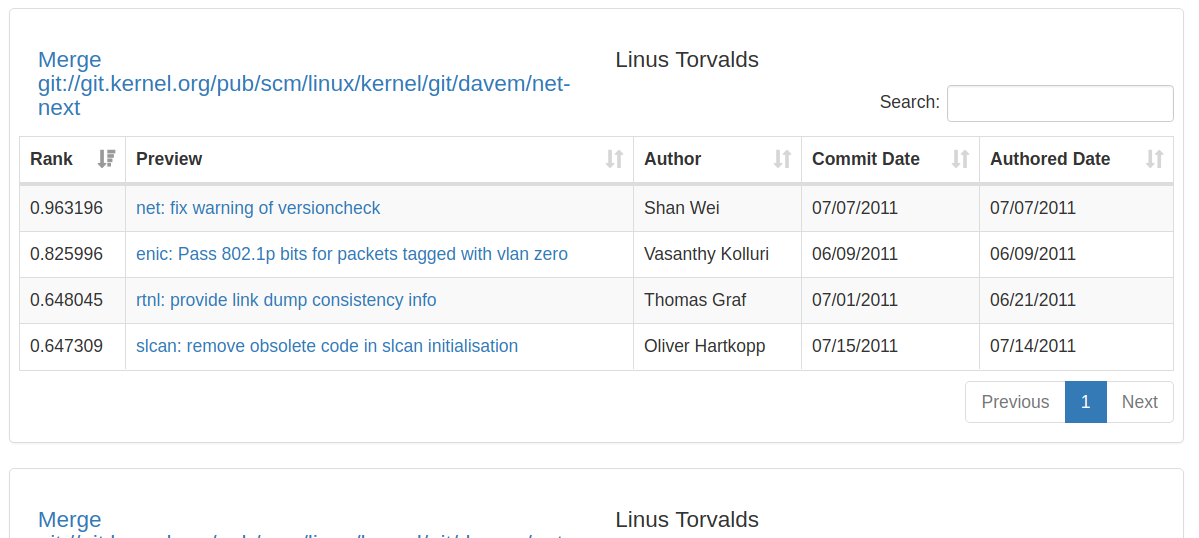
\includegraphics[width=\linewidth]{figures/linvis/search_results.png}
  \caption{A single \mt tree in the search results of \tool, showing
    the link to the root at the top and a table of the relevant commits
    in the bottom, sorted by relevance.}
  \label{fig:search_results}
\end{figure}

Before presentation, the results are grouped by \mt root. Each group
has a link to the root-node of the tree at the top, followed by a table
of commits and merges within the tree that match the query, shown in
Figure~\ref{fig:search_results}. The table includes the relevancy rank
of the entry, the commit log message preview, author, the date the
repository event was committed, and the date it was authored. The merge
tree groups are ordered based on the mean of the relevancy scores of the
relevant results in that tree.

\subsection{Summarization}
\label{sub:summarization}

\tool uses seven tabs to show the information and visualizations for a
selected repository event. The summarization tabs are; messages, files, modules,
authors; the visualization tabs are; list tree, pack tree, and \rt tree.

The message tab shows the full commit log message. This does not include
the diff, but given the commit hash, this information can be found
directly from the repository.

The files tab shows an aggregated table of all files that were modified
in a merge. It includes metrics like the number of lines added, lines
removed, total lines modified, and the delta, summed across all commits
in the \mt tree that modify this file. A details drop-down button
allows a user to see exactly which commit makes the changes, as shown in
Figure~\ref{fig:linvis_files}. If the current repository event being
viewed is a commit, the aggregate views will only show modifications
made by the commit.

The modules tab shows the modules modified in the \mt. Like the
files tab, the modules tab uses a table to show the name of the module,
the number of commits that are in the \mt tree that work with the
module, and a details button to provide the links to those commits.

\begin{figure}[htpb]
  \centering
  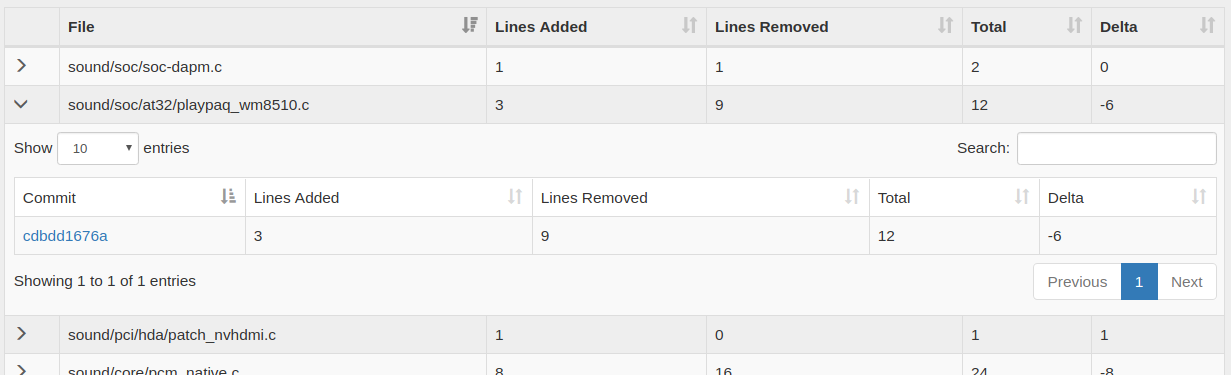
\includegraphics[width=\linewidth]{figures/linvis/linvis_files.png}
  \caption{Table showing the modified files in a merge, with the second
  entry expanded to show the commit that makes the changes.}
  \label{fig:linvis_files}
\end{figure}

The authorship tab is very similar to the files tab, but shows the
authorship information. It shows the sum of the number of lines added,
removed, modified, and the delta within the \mt. It also shows the
number of files that were modified by the author. The details tab is
organized slightly differently. Instead of organizing the results by
commit, the details are organized by file, showing which files were
modified by the author in this \mt (Figure~\ref{fig:linvis_authors}).

\begin{figure}[htpb]
  \centering
  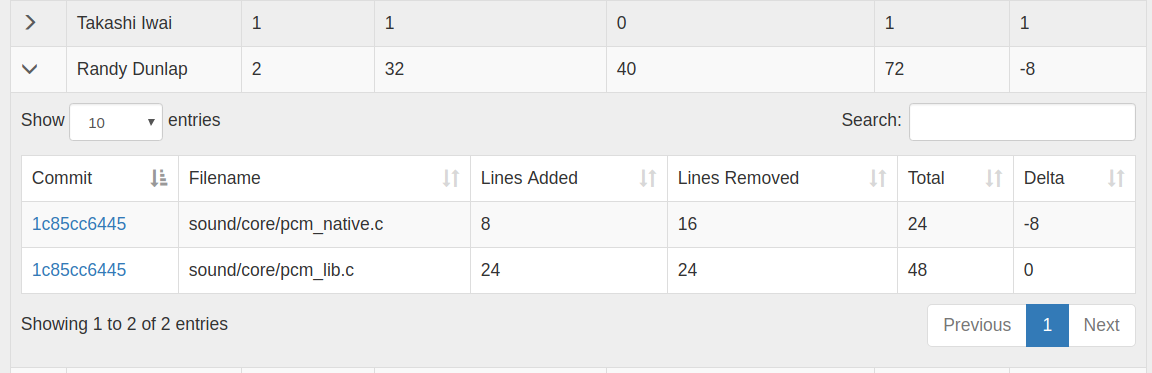
\includegraphics[width=\linewidth]{figures/linvis/linvis_authors.png}
  \caption{Table showing the authors who made changes in a merge. The
    entry for Randy Dunlap is expanded, showing the modifications to
    each file that were made by Randy.}
  \label{fig:linvis_authors}
\end{figure}


\subsection{Visualization}
\label{sub:visualization}

The ability to easily visualize the integration of commits into a
project is what makes \tool unique from other tools. \tool implements
three visualizations, the list tree, pack tree, and \rt tree.

\subsubsection{List Tree}

The list tree, depicted in Figure~\ref{fig:linvis_list_tree}, is
constructed as a series of nested lists. The nesting indicates the
parent-child relationship. This visualization is text-based enabling
fast navigation to commits using the built-in search in most
web-browsers. The list tree is rooted at the current repository event;
if the current event being inspected is a commit, only that commit will
be shown. Conversely, if the selected event is the root, the entire
\mt tree will be shown.

\begin{figure}
        \centering
        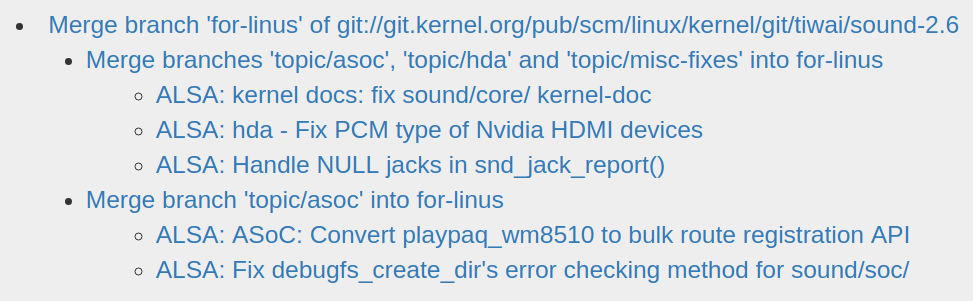
\includegraphics[width=0.9\linewidth]{figures/linvis/linvis_list_tree.png}
        \caption{The list tree visualization}
        \label{fig:linvis_list_tree}
\end{figure}

\subsubsection{\rt Tree}

The \rt tree\cite{Reingold1981}, depicted for two trees in
Figure~\ref{fig:study_commits}, is the classic tree visualization, with
the root at the top, leaves at the bottom, and edges between them
showing the parent-child relationship. This tree visualization works
very well in many cases, but does not easily visualize very wide trees,
with many repository events on a single level.

When a user first looks at the visualization, the current repository
event is placed in the center. Furthermore, it is highlighted in bright
orange. Commits, the leaves, are shown in white, while the merges are
colored shades of blue where lighter blue indicates fewer child events
of that node, and darker blue indicates more children.

\subsubsection{Pack Tree}

Pack trees\cite{Wang2006} are useful for displaying an overview of large
data sets. The initial goal for the pack tree was for visualizing file
systems, which are similar to git repositories in that they are
relatively shallow, but very wide trees. The tree is represented by sets
of nested circles. The largest circle, containing all of the other
nodes, is the root, while the smallest circles are the leaves. In our
representation, the root maps to the merge into the master branch, while
the leaves are the commits.


\begin{figure}[htpb]
  \centering
  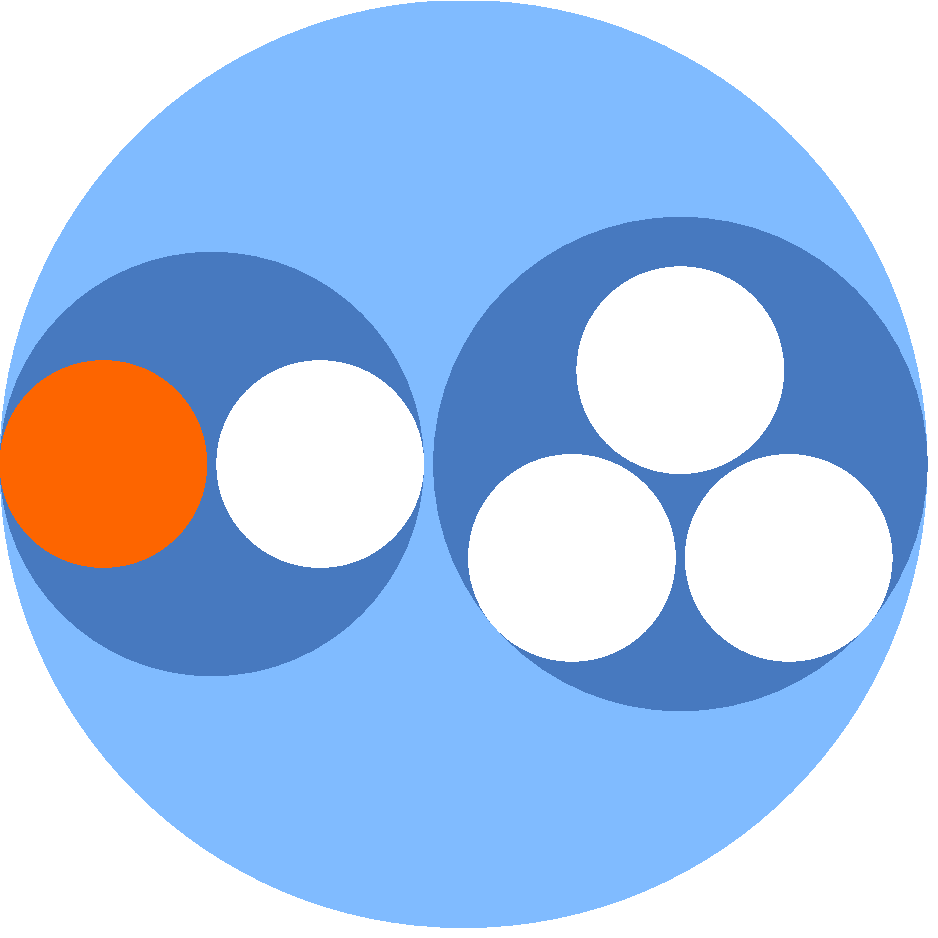
\includegraphics[width=0.8\linewidth]{figures/linvis/linvis_bubble.pdf}
  \caption{The pack tree visualization, with the root depicted as the
    outer-most circle, containing all other nodes, the leaves depicted
    as white circles containing no other nodes. The currently selected
    event is shown in orange.}
  \label{fig:linvis_pack}
\end{figure}

We depict the pack tree in Figure~\ref{fig:linvis_pack}. Like with the
\rt tree, \tool uses white to indicate the individual commits, and
orange to indicate the currently selected node. The inner merges are
colored with shades of blue to indicate the depth in the tree. Darker
shades of blue indicate that the merge is deeper in the tree; the root
will be the lightest shade.


\section{Related Works}
\label{sec:related_works}

% vim:set et sw=2 ts=4 tw=72:
% Jul 04, 2017
% Evan Wilde

\section{Related Works}
\label{sec:related_works}

Version control systems monitor the development lifetime of software
projects. This makes the version control system vital in providing
information about how a software project is being developed. To do this,
the user must be able to gain a clear understanding of how commits are
being integrated into the project, along with understanding what changes
these commits are bringing with them. These are the tasks that we set
out to solve with the \mt model. Ideally, we could compare our model
against another that is designed with these goals. To our knowledge, we
know of no git repository visualization tool that has these specific
goals. This may be due to issues with finding the master branch of the
repository which is a non-trivial task, or due to other factors. While
we have found no tool with the express goal of showing how a commit is
integrated, and providing a summarization of a merge, there has been a
lot of work done in providing visualizations of various aspects of a
repository.

Many tools work to address the issues in communication between
developers in inter-team collaboration work. Codebook\cite{Begel2010}
uses a data mining technique to determine the developer of a piece of
code, the program manager who wrote the specification for the code, and
the program managers and developers on the team who were working
together. Hipikat\cite{Cubranic2005} is another tool with a focus on
communication. Where Codebook focuses on developers working on a
project, Hipikat is focused on enabling easier integration of new
developers to a project by providing them with easily-searchable
artifacts of the changes made. Codebook is useful for pairing a
contributor with the original developer; however, the developer may not
have worked with the piece of code in years. A Hipikat program may
provide more information to the maintainer as it records the artifacts
of why certain design decisions were made when they were made using
other tools like Bugzilla and CVS.\@ Neither tool is sufficient in
meeting our goals to provide a summary of the topology of the kernel
repository through a visual tree.

Most visualizers provide a visual presentation of a certain aspect of a
repository. Fractal Figures\cite{Ambros2005} uses a unit square to
represent a portion of a project, then partitions the square based on
the proportion of an author's contributions to that portion of the
project. EPOSee\cite{Burch2005} and Evolution Radar\cite{Ambros2009}
perform further analysis, determine which files are made together, and
what changes are made over a sequence of commits, though the goals
behind these projects is different.

Codebook, Hipikat, Fractal Figures, EPOSee, and Evolution Radar all work
with data from CVS repositories. Our goal is to provide information
about Git repositories, specifically the Linux master repository. Fewer
tools are available for generating visualizations and summaries of Git
repositories, potentially due to the DAG model used by Git.

Gource is a tool for providing an interactive timelapse of the state of
a repository\cite{Caudwell2010}. In the timelapse, it shows who
contributes and what type of contribution a developer is making. These
contribution types are one of, adding a file, removing a file, and
changing a file. While the timelapse is interesting to watch, it does
not provide any additional explanation of the changes actually being
made, only the frequency that they are being made and who is making
them. Codeswarm\cite{ogawa09} is similar to Gource, using an organic approach to
visualizing events in the repository. Unlike Gource, which focuses on
the files, Codeswarm focuses on developers and the number of commits
they are making.

Git itself is shipped with summarization and visualization tools: the
\verb|git log| command and Gitk, which is a graphical tool for the
purpose of browsing the DAG of the repository. Many other tools are
designed with a similar visual metaphore as what is presented in Gitk,
including GitKraken, Github Desktop and web interfaces, the Git Lab web
interface, the Bitbucket web interface, are a few examples. The Gitk
interface is built around the central DAG viewer. The DAG displays the
repository events on their respective branches, the author, and the date
that the event was authored. A user can select an event to view addition
information about it, including the full commit log, the parents and
children of the event, and the diff generated if modifications were
made. In the case of the Linux kernel, merges are not resolved as merge
conflicts in the master repository, but by the developers prior to
merging through rebase operations. With this development model, no
merges will have modified any files, and will not show a diff. While the
merge does not make changes directly, the effects of merging the commits
persist, but Gitk is unable to provide an aggregated view of the files
modified, the patches for those files, and the authors who contributed
commits to that merge.

Our tool is primarily aimed at presenting the hierarchical structure of
the Linux git repository. We use tables for presenting the summarized
information of the commits and merges, but this information could also
be presented in a graphical form. Various graphical forms for displaying
file and authorship data exist, the principal forms being matrix views,
city scapes, bar and pie charts, and networks \cite{Eick2002}. Any of
these data visualization metaphors are applicable to our system.

%%% Local Variables:
%%% mode: latex
%%% TeX-master: "lineval.tex"
%%% End:


\section{Controlled User Study}
\label{sec:study}

\section{Controlled User Study}
\label{sec:study}

We conducted a study to quantitatively and qualitatively evaluate the
effectiveness of \tool compared to the DAG-based visualizations found in
Gitk or the git command line. The study is broken into three task-based
sections; conceptual tasks, summarization tasks, and participant
opinions. The study was performed during June of 2017 in a controlled
environment running Ubuntu 14.04. To evaluate the DAG-based
visualizations, participants were allowed to use both Gitk and the git
command-line tools together, which we will refer to as Gitk. \tool was
used for evaluating \mt-based visualizations.

The primary goal of the study is two fold; first determining if the
DAG-based visualization is sufficient for conceptual understanding;
second comparing \tool and Gitk to determine which is more capable of
providing users with a summarization of various metrics involved with
integrating a commit into the repository. The conceptual questions are
to determine if the DAG-based visualizations (Gitk and git command line)
provide enough information to determine how a commit, and any related
commits, are merged into a project. \tool displays this information
directly in the form of a tree, so we will not be performing a
comparison on this section, only evaluating the results from Gitk. The
summarization tasks compare \tool and Gitk, with the participants using
one tool followed by the other on two commits from \mt{s} of
differing sizes. In both of these sections, the participant is given a
task that they are to find an answer to; we evaluate the time it took,
if the answer was correct, and how far from the right answer they were.
The user opinions provide us with a clear comparison between the tools
from the point-of-view of the participant, providing us information
about which aspects of each tool they preferred.

\subsection{Tasks}
\label{sub:tasks}

\begin{table*}[htpb]
  \centering
  \caption{Conceptual Tasks }
  \label{tab:conceptual_tasks}
  \begin{tabulary}{0.9\textwidth}{LL}
    \toprule
    Task & Description\\
    \midrule
    T1 & Draw a diagram showing how this commit was merged into the master branch, along with any other related commits\\
    T2 & How many individual commits are related to this commit?\\
    T3 & How many merges are involved with merging this commit into the master branch?\\
    \bottomrule
  \end{tabulary}
\end{table*}

\begin{table}[htpb]
  \centering
  \caption{Summarization Tasks}
  \label{tab:summarization_tasks}
  \begin{tabulary}{\linewidth}{LLL}
    \toprule
    Task Set   & Task & Description\\\midrule
    Merge      & T4   & What is the series of merges involved with merging this
    commit?\\
    & T5   & What other commits are merged?\\
    Authorship & T6   & How many authors are involved?\\
    & T7   & Who contributed the most changes?\\
    Files      & T8   & How many files were modified?\\
    & T9   & Which file had the most changes?\\
    Modules    & T10  & Which modules does this \mt involve?\\
    \bottomrule
  \end{tabulary}
\end{table}


\textbf{The conceptual tasks} are designed to gain better insight on the
comprehension of the visualization in Gitk, and determine if it is
sufficient for understanding what other commits are related to a given
commit, and how those commits are merged. The tasks are outlined in
Table~\ref{tab:conceptual_tasks}. The tasks are performed in order using
Gitk. T1 has the participant draw a diagram of the \mt,
which will be used to answer the other two questions. This enables us to
see issues with comprehending the DAG visualization. Participants are
given 10 minutes to perform this task, which also is used to familiarize
the participant with the Gitk interface, if they are not already, and
with the set of commits they will be working with. T2 and T3 are drawn
directly from the diagram from T1, giving quantitative metrics to
measure the comprehension. T2 asks the participant to verify the number
of commits, and T3 asks for the number of merges. The three tasks are
performed on both commits before continuing to the summarization tasks.


\textbf{The summarization tasks}, listed in
Table~\ref{tab:summarization_tasks}, are designed to compare the ability
of the participants to summarize information about the two commits used
in the study when using Gitk versus \tool. The tasks are broken into
four sets based on what is being summarized: merges, authorship, files,
and modules. The order that the participants perform each task is
randomized within each task set, and the order of the task sets are then
randomized with the exception of the merge task set which will always
come first. The order that the tools are used is kept consistent for a
participant, but randomized between participants. We measure and
evaluate three metrics for each task: correctness, accuracy, and timing.
Correctness measures whether the answer was correct or incorrect.
Accuracy measures how far from being correct the provided answer was.
Timing is the duration, in seconds, that the participant took to answer
the task. We begin timing the task at the end of the question, and stop
timing before the last modification to the answer. For this reason, it
is possible for times to overlap between tasks if the participant
changes their answer after answering another question. This will also
modify the answer used for measuring the accuracy. We measure the timing
from the screen capture.

While the merge task set is part of the summarization task group, it
focuses less with summarization of the commits and more with
comprehension of the model visualizations. The task is designed with two
goals in mind; first we want to measure and define which commits and
which merges the participant has defined to be in the \mt; second
to help solidify which commits and merges will be used in the merge
tree.

T4 provides a concrete series of merges that the participant believes to
be integrating the commit into the repository. T5 provides a concrete
set of commits that are related to the commit. We place these tasks
first as the answers to these will be necessary for the participant to
answer the tasks that follow, specifically finding the merge into the
master branch. T6 and T7 are related to the authorship of a merge,
determining how many authors are involved and who made the most changes.
T8 and T9 are related to the files that were modified in the merge,
determining how many files were modified and which file had the most
changes. T10 is related to the modules that were modified in the merge.
Modules are not explicitly defined in git, but are a property of the
Linux repository that we noticed while looking at various commits. To
find the module name, take the text up to the first colon in the git log
preview. For the log preview \textit{``ALSA: kernel docs: fix
  sound/core/ kernel-doc''} the module is \textit{``ALSA''}, e.g.

The correctness metric is simply whether the answer was correct or not;
an accuracy of zero indicates a correct answer. The accuracy metrics are
measured slightly differently between tasks due to different
requirements and structures in the answer. In task T4, both the order
and the merges are important. We define the distance to be the edit
distance with insertion, deletion, and transposition at unit cost. The
accuracy is the minimum edit distance necessary to make the answer
correct. T5, T9, and T10 are concerned with the set of elements in the
response; the order is not important. We use the Levenshtein distance,
with insertion, deletion, and substitution operations of unit cost, from
the provided answer to the correct answer. The answers to T6 and T8 are
single number values; the distance is measured as the absolute value of
the difference between the provided answer and the correct answer. T7
has only a single correct answer, thus the distance would either be zero
or one. For this reason, it is acceptable to omit the accuracy metric
from this task.

Statistical significance testing is performed to verify that the results
are meaningful. We use $alpha = 0.05$ or a $95\%$ confidence level. The
McNemar $\chi^2$ test\cite{McNemar1947} with continuity correct is used
to test the statistical significance of the hypothesis that \tool
improves correctness of the participants. The $\chi^2$ threshold
statistic at $\alpha = 0.05$ is 3.841. The Wilcoxon\cite{Wilcoxon45}
test and Cliff's effect size\cite{Cliff93} are applied to the accuracy
and timing metrics to determine the significance of the difference
between \tool and Gitk. The Wilcoxon test is applied between commits to
determine if the size of the \mt effects timing and accuracy. The
null hypotheses and alternative hypotheses are stated in
Table~\ref{tab:null_alt_hypoths}.

\begin{table*}[h!]
  \centering
  \caption{Null and Alternative Hypotheses for Summarization Tasks\evan{Should I say exactly
      what the null hypotheses are referring to (counting authors,
      files, etc... or is this good enough? It's already a huge and
      redundant table) }}
  \label{tab:null_alt_hypoths}
  \begin{tabulary}{0.98\linewidth}{CCLL}
    \toprule
    Task & Metric             & Null Hypothesis                                                      & Alternative Hypothesis\\\midrule
    T4   & \tiny{Commit}      & There is no difference on accuracy or timing between \comA and \comB & There is a difference on accuracy or timing between \comA and \comB \\
    T4   & \tiny{Correctness} & \tool does not effect the correctness of the participants            & \tool does effect the correctness of the participants\\
    T4   & \tiny{Accuracy}    & There is no difference between \tool and Gitk on accuracy            & There is a difference between \tool and Gitk on accuracy\\
    T4   & \tiny{Timing}      & There is no difference between \tool and Gitk on timing              & There is a difference between \tool and Gitk on timing\\

    T5   & \tiny{Commit}      & There is no difference on accuracy or timing between \comA and \comB & There is a difference on accuracy or timing between \comA and \comB \\
    T5   & \tiny{Correctness} & \tool does not effect the correctness of the participants            & \tool does effect the correctness of the participants\\
    T5   & \tiny{Accuracy}    & There is no difference between \tool and Gitk on accuracy            & There is a difference between \tool and Gitk on accuracy\\
    T5   & \tiny{Timing}      & There is no difference between \tool and Gitk on timing              & There is a difference between \tool and Gitk on timing\\

    T6   & \tiny{Commit}      & There is no difference on accuracy or timing between \comA and \comB & There is a difference on accuracy or timing between \comA and \comB \\
    T6   & \tiny{Correctness} & \tool does not effect the correctness of the participants            & \tool does effect the correctness of the participants\\
    T6   & \tiny{Accuracy}    & There is no difference between \tool and Gitk on accuracy            & There is a difference between \tool and Gitk on accuracy\\
    T6   & \tiny{Timing}      & There is no difference between \tool and Gitk on timing              & There is a difference between \tool and Gitk on timing\\

    T7   & \tiny{Commit}      & There is no difference on accuracy or timing between \comA and \comB & There is a difference on accuracy or timing between \comA and \comB \\
    T7   & \tiny{Correctness} & \tool does not effect the correctness of the participants            & \tool does effect the correctness of the participants\\
    T7   & \tiny{Accuracy}    & There is no difference between \tool and Gitk on accuracy            & There is a difference between \tool and Gitk on accuracy\\
    T7   & \tiny{Timing}      & There is no difference between \tool and Gitk on timing              & There is a difference between \tool and Gitk on timing\\

    T8   & \tiny{Commit}      & There is no difference on accuracy or timing between \comA and \comB & There is a difference on accuracy or timing between \comA and \comB \\
    T8   & \tiny{Correctness} & \tool does not effect the correctness of the participants            & \tool does effect the correctness of the participants\\
    T8   & \tiny{Accuracy}    & There is no difference between \tool and Gitk on accuracy            & There is a difference between \tool and Gitk on accuracy\\
    T8   & \tiny{Timing}      & There is no difference between \tool and Gitk on timing              & There is a difference between \tool and Gitk on timing\\

    T9   & \tiny{Commit}      & There is no difference on accuracy or timing between \comA and \comB & There is a difference on accuracy or timing between \comA and \comB \\
    T9   & \tiny{Correctness} & \tool does not effect the correctness of the participants            & \tool does effect the correctness of the participants\\
    T9   & \tiny{Accuracy}    & There is no difference between \tool and Gitk on accuracy            & There is a difference between \tool and Gitk on accuracy\\
    T9   & \tiny{Timing}      & There is no difference between \tool and Gitk on timing              & There is a difference between \tool and Gitk on timing\\

    T10   & \tiny{Commit}      & There is no difference on accuracy or timing between \comA and \comB & There is a difference on accuracy or timing between \comA and \comB \\
    T10   & \tiny{Correctness} & \tool does not effect the correctness of the participants            & \tool does effect the correctness of the participants\\
    T10   & \tiny{Accuracy}    & There is no difference between \tool and Gitk on accuracy            & There is a difference between \tool and Gitk on accuracy\\
    T10   & \tiny{Timing}      & There is no difference between \tool and Gitk on timing              & There is a difference between \tool and Gitk on timing\\
    \bottomrule
  \end{tabulary}
\end{table*}


\textbf{The user-opinion} questions, listed in
Table~\ref{tab:opinion_questions}, are designed to determine which tool
provides a better user experience for summarization and comprehension
tasks, and what aspects of each assisted with their understanding. T11
asks for the preference of the participant, given that their goal is
comprehension and summarization. % TODO add T11 results
We recognize that neither tool is perfect, and participants may have
complaints about both tools, but are interested in what parts of each
tool assisted them with understanding the events in the repository. T12
is meant to address this. % TODO add T12 results


\begin{table}[htpb]
  \centering
  \caption{User-Opinion Questions}
  \label{tab:opinion_questions}
  \begin{tabulary}{0.9\linewidth}{LL}
    \toprule
    Task & Description\\
    \midrule
    T11 & Given these tasks again, which tool would you prefer?\\
    T12 & Which aspects of each tool did you like and why?\\
    \bottomrule
  \end{tabulary}
\end{table}


\subsection{Commit Selection}
\label{sub:commit_selection}

We include two commits in the study to detect differences in the
correctness, accuracy, and timing between \mt sizes. The order that the
commits are presented to each participant is randomized. We analyzed the
15096 \mt{s} from April 16th 2005 to October 14th 2014, which
corresponds to the releases Linux 2.6.12-rc3 and Linux 3.17-rc1. 25\% of
the trees contain at most a single commit not including the root, while
50\% of the trees contain at most seven non-root nodes. 75\% of the
trees contain at least 51 nodes, and the largest tree contains 7217
nodes.

From this information, we selected one tree with a single commit, and
one tree with seven non-root nodes to represent a small tree and a
medium-sized tree. A majority of the trees are flat, where all nodes
merge directly into the root node. Of the 8031 trees containing at least
seven non-root nodes, only 593 contained at least a single internal
merge node. Trivially, trees with a single node cannot have any internal
nodes, and of the 624 trees with seven non-root nodes, only 135
contained at least one inner node. To increase the complexity of the
medium-sized tree, we randomly selected one of the 135 trees to
represent the medium tree.

From the 2008 trees containing only a single node, we selected one at
random, and trivially selected the only commit in the tree. From the
trees containing seven non-root nodes, we selected one tree randomly,
then randomly selected one of the commits in the tree. We selected
commit \emph{a3c1239eb59c0a907f8be5587d42e950f44543f8} from the tree
containing a single node, which we will refer to as \comA, and commit
\emph{cdbdd1676a5379f1d5cbd4d476f5e349f445befe} from the tree containing
seven nodes, which we will refer to as \comB. A visual representation
for these trees is shown in Figure~\ref{fig:study_commits}.

\begin{figure}[bpt]
  \centering
  \begin{tabular}{ m{1.5cm} m{3cm} }
    
\includegraphics[height=0.5in]{figures/commits/1-commit.pdf} &
    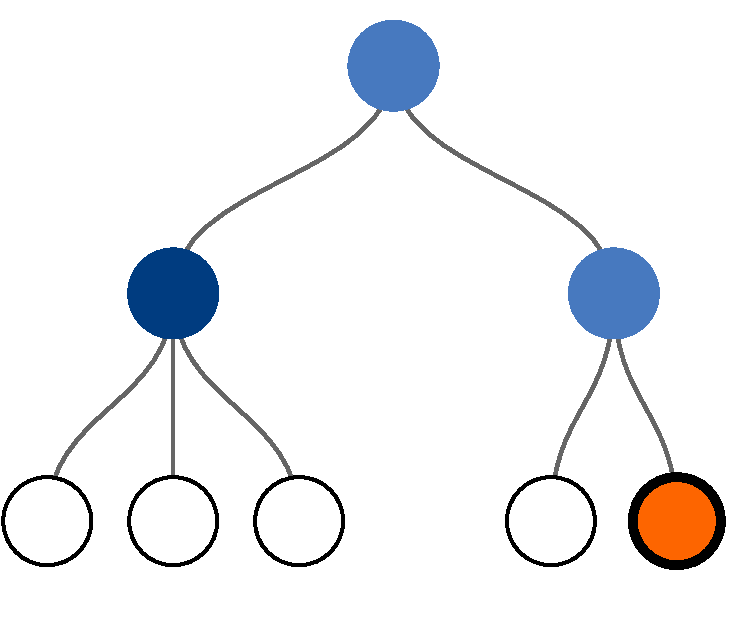
\includegraphics[height=1in]{figures/commits/7-commits.pdf}\\
  \end{tabular}
  \caption{The \mt{s} used in the user study,
    containing one and seven non-root nodes, respectively.}
  \label{fig:study_commits}
\end{figure}

\subsection{Participant Profile}
\label{sub:participant_profile}

The study was conducted with 12 participants, all of whom were masters,
PhD, or post-doc researchers in the field of software engineering. The
participants had between 6 months and 10 years experience with git, with
the median being 3.5 years. Most participants had additional experience
with SVN and CVS.\@ One of the participants in the study worked as a
release engineer, studying merge practices to determine the best way to
merge branches while minimizing the number of merge conflicts, on SVN
repositories. The participants worked with repositories ranging from
around 10 commits up to 38000 commits, with the median being 350
commits. Two of the participants had never collaborated with anyone in a
repository, while the rest had some experience with repositories being
modified by multiple people, with the most being 219. The median number
of collaborators was four. Participants had most experience with
personal and academic repositories. Three of the twelve participants had
experience with professional repositories.

All participants have had at least some experience with version control,
branching in repositories, and git. The participants are from the same
lab, and each participant worked with both tools in the study, thus,
keeping the sample populations identical for both tools, with some
variation between participants in experience with repositories.

\subsection{Study Procedure}
\label{sub:study_procedure}

The study begins with a short introduction to the \mt model, followed by
an introduction to Gitk and \tool. We provided two examples of
converting the DAG to the \mt. The first example DAG was a flat merge,
so the corresponding \mt did not have any internal nodes. The
second was not a flat merge, so the corresponding \mt contained a
single internal node. Any questions about the model were answered at
this time. Following the introduction to the \mt model, we introduce
Gitk and \tool, providing information about what each pane shows in
Gitk, and what each tab does in \tool.

The conceptual tasks follow the introduction, followed by the
summarization, which are then followed by the user opinion. The study is
concluded with three questions to enable us to learn more about the
participants;

\begin{itemize}
  \item How long have you used git?
  \item For what kind of projects have you used git?
  \item How many commits, files, and collaborators were involved with
    the largest repository you have worked with?
\end{itemize}

To mitigate the order bias cased by using one tool before the other or
one commit before the other, we randomize both the order that the tools
are used, and the order that the commits are used, between participants.
The conceptual tasks are run twice, once with \comA and once with \comB,
in the same order for all participants using the Gitk.

\evan{This paragraph is kind of tricky to explain well. See if you can
  understand what I'm trying to say} The summarization tasks are run
four times, once with \comA and \tool, \comB and \tool, \comA and git
tools, and \comB and Gitk. The participant will start with one
tool, and complete the tasks for both commits in that tool. The order of
the commits is the same as in the conceptual tasks. Once they complete
the summarization tasks for both \comA and \comB, they will switch to
the other tool and complete the tasks again on the commits in the same
order. The order of the tasks is consistent over all four runs. The
questions in the user opinions section do not directly involve the tools
or commits.

We use a script written in python 3.6.1 in order to assure that we do
not bias the randomization, and ensure that correct ordering is
maintained between tools, tasks, and commits. The script produces the
entire script for the study, so we only need to read it to correctly
conduct the study. Re-running the script generates the study for the
next participant. We use screen capture to record the audio and video.
From the screen capture, we measure the time, as well as recording the
responses in the study.

\evan{Should I include the python script? It would make explaining how
  the test was conducted 100\% clear.}
\evan{I think it would be far too long then.}

\subsection{Results}
\label{sec:results}

\evan{This looks weird not having text between the subsections... Should
  I put something here?...}

\subsubsection{Conceptual Tasks}
\label{sub:conceptual_tasks}

Table~\ref{tab:conceptual_results} shows a summary of the results from
conceptual tasks T2 and T3. The answer column contains the correct
answer to the corresponding task, while the median, mean, and variance
columns are with respect to the answers provided by the
participants.\evan{Is this better for describing the columns in the
  table?} The median(s), mean(s), and variance(s) columns are with
respect to the time taken, in seconds, by the participants to respond to
the tasks.

\evan{Should I add some of the drawings to the paper?}

The results from T1 did not vary greatly between the participants. The
drawings generally show something in the form of a list, starting from
the provided commit and traversing the master branch, indicating that
the participants were unable to determine which merge was in the master
branch. Many of the participants identified the next tag, v2.6.29-rc6,
to be ``the master branch'', however, a tag is not a branch. One
participant was able to draw the correct diagram for \comA directly
from the git command line, but rejected their response after inspecting
the DAG visualization provided by Gitk and proceeded to draw a list of
merges.


\begin{table*}[htpb]
  \centering
  \caption{Results from the conceptual questions}
  \label{tab:conceptual_results}
  \begin{tabular}{ll|r|lrr|rrr}
    Question & Commit & Answer & Median & Mean  & Variance & Median(s) & Mean(s) & Variance(s)\\\hline\hline
    T2       & \comA  & 1      & 4      & 19.11 & 753.11   & 10.0      & 49.92   & 5952.08\\
    T3       & \comA  & 1      & 5      & 8.27  & 53.62    & 7.5       & 24.67   & 884.42\\\hline
    T2       & \comB  & 5      & 4      & 7.80  & 136.84   & 31.5      & 106.83  & 54123.42\\
    T3       & \comB  & 3      & 3.5    & 5.40  & 50.27    & 11.0      & 65.6    & 29798.82\\
  \end{tabular}
\end{table*}

Users were able to more closely estimate the number of commits and
merges in the larger tree, but generally took longer than the smaller
tree. The tree with a single node resulted in more variability in the
estimate of number of commits. It should be noted that these questions
were answered after spending roughly ten minutes attempting to draw a
picture that held the answers to these questions, so the times indicate
how quickly the participant was able to interpret their conceptual
understanding.

\subsubsection{Summarization Tasks}
\label{sub:summarization_tasks}

Table~\ref{tab:cross_commit_results} shows whether the \mt size
has an effect on the three studied metrics. An interesting observation
from the figure is that the correctness for T5 and T9 are effected by
the size of the \mt, but the accuracy is not. The correctness
results for T5 and T9 are shown in Figure~\ref{fig:correctness_t5_t9},
and the timing results for T7 are shown in Figure~\ref{fig:timing_t7}.

\begin{table}[htpb]
  \centering
  \caption{Cross-Commit Results\evan{Should I group the results by task
      or by metric? It's by metric right now}}
  \label{tab:cross_commit_results}
  \begin{tabular}{ccrl}
    \toprule
    Task & Metric      & $p$-value & Conclusion\\\midrule
    T4   & Correctness & 0.22      & Do not reject $H_0$\\
    T5   & Correctness & 0.04      & Reject $H_0$\\
    T6   & Correctness & 0.13      & Do not reject $H_0$\\
    T7   & Correctness & 0.06      & Do not reject $H_0$\\
    T8   & Correctness & 0.07      & Do not reject $H_0$\\
    T9   & Correctness & 0.04      & Reject $H_0$\\
    T10  & Correctness & 0.62      & Do not reject $H_0$\\

    T4  & Accuracy & 0.94 & Do not reject $H_0$\\
    T5  & Accuracy & 0.09 & Do not reject $H_0$\\
    T6  & Accuracy & 0.19 & Do not reject $H_0$\\
    T8  & Accuracy & 0.16 & Do not reject $H_0$\\
    T9  & Accuracy & 0.08 & Do not reject $H_0$\\
    T10 & Accuracy & 0.37 & Do not reject $H_0$\\

    T4  & Time & 0.77 & Do not reject $H_0$\\
    T5  & Time & 0.97 & Do not reject $H_0$\\
    T6  & Time & 0.90 & Do not reject $H_0$\\
    T7  & Time & 0.01 & Reject $H_0$\\
    T8  & Time & 0.87 & Do not reject $H_0$\\
    T9  & Time & 0.99 & Do not reject $H_0$\\
    T10 & Time & 0.68 & Do not reject $H_0$\\
    \bottomrule
  \end{tabular}
\end{table}

\begin{figure*}[htpb]
  \centering
  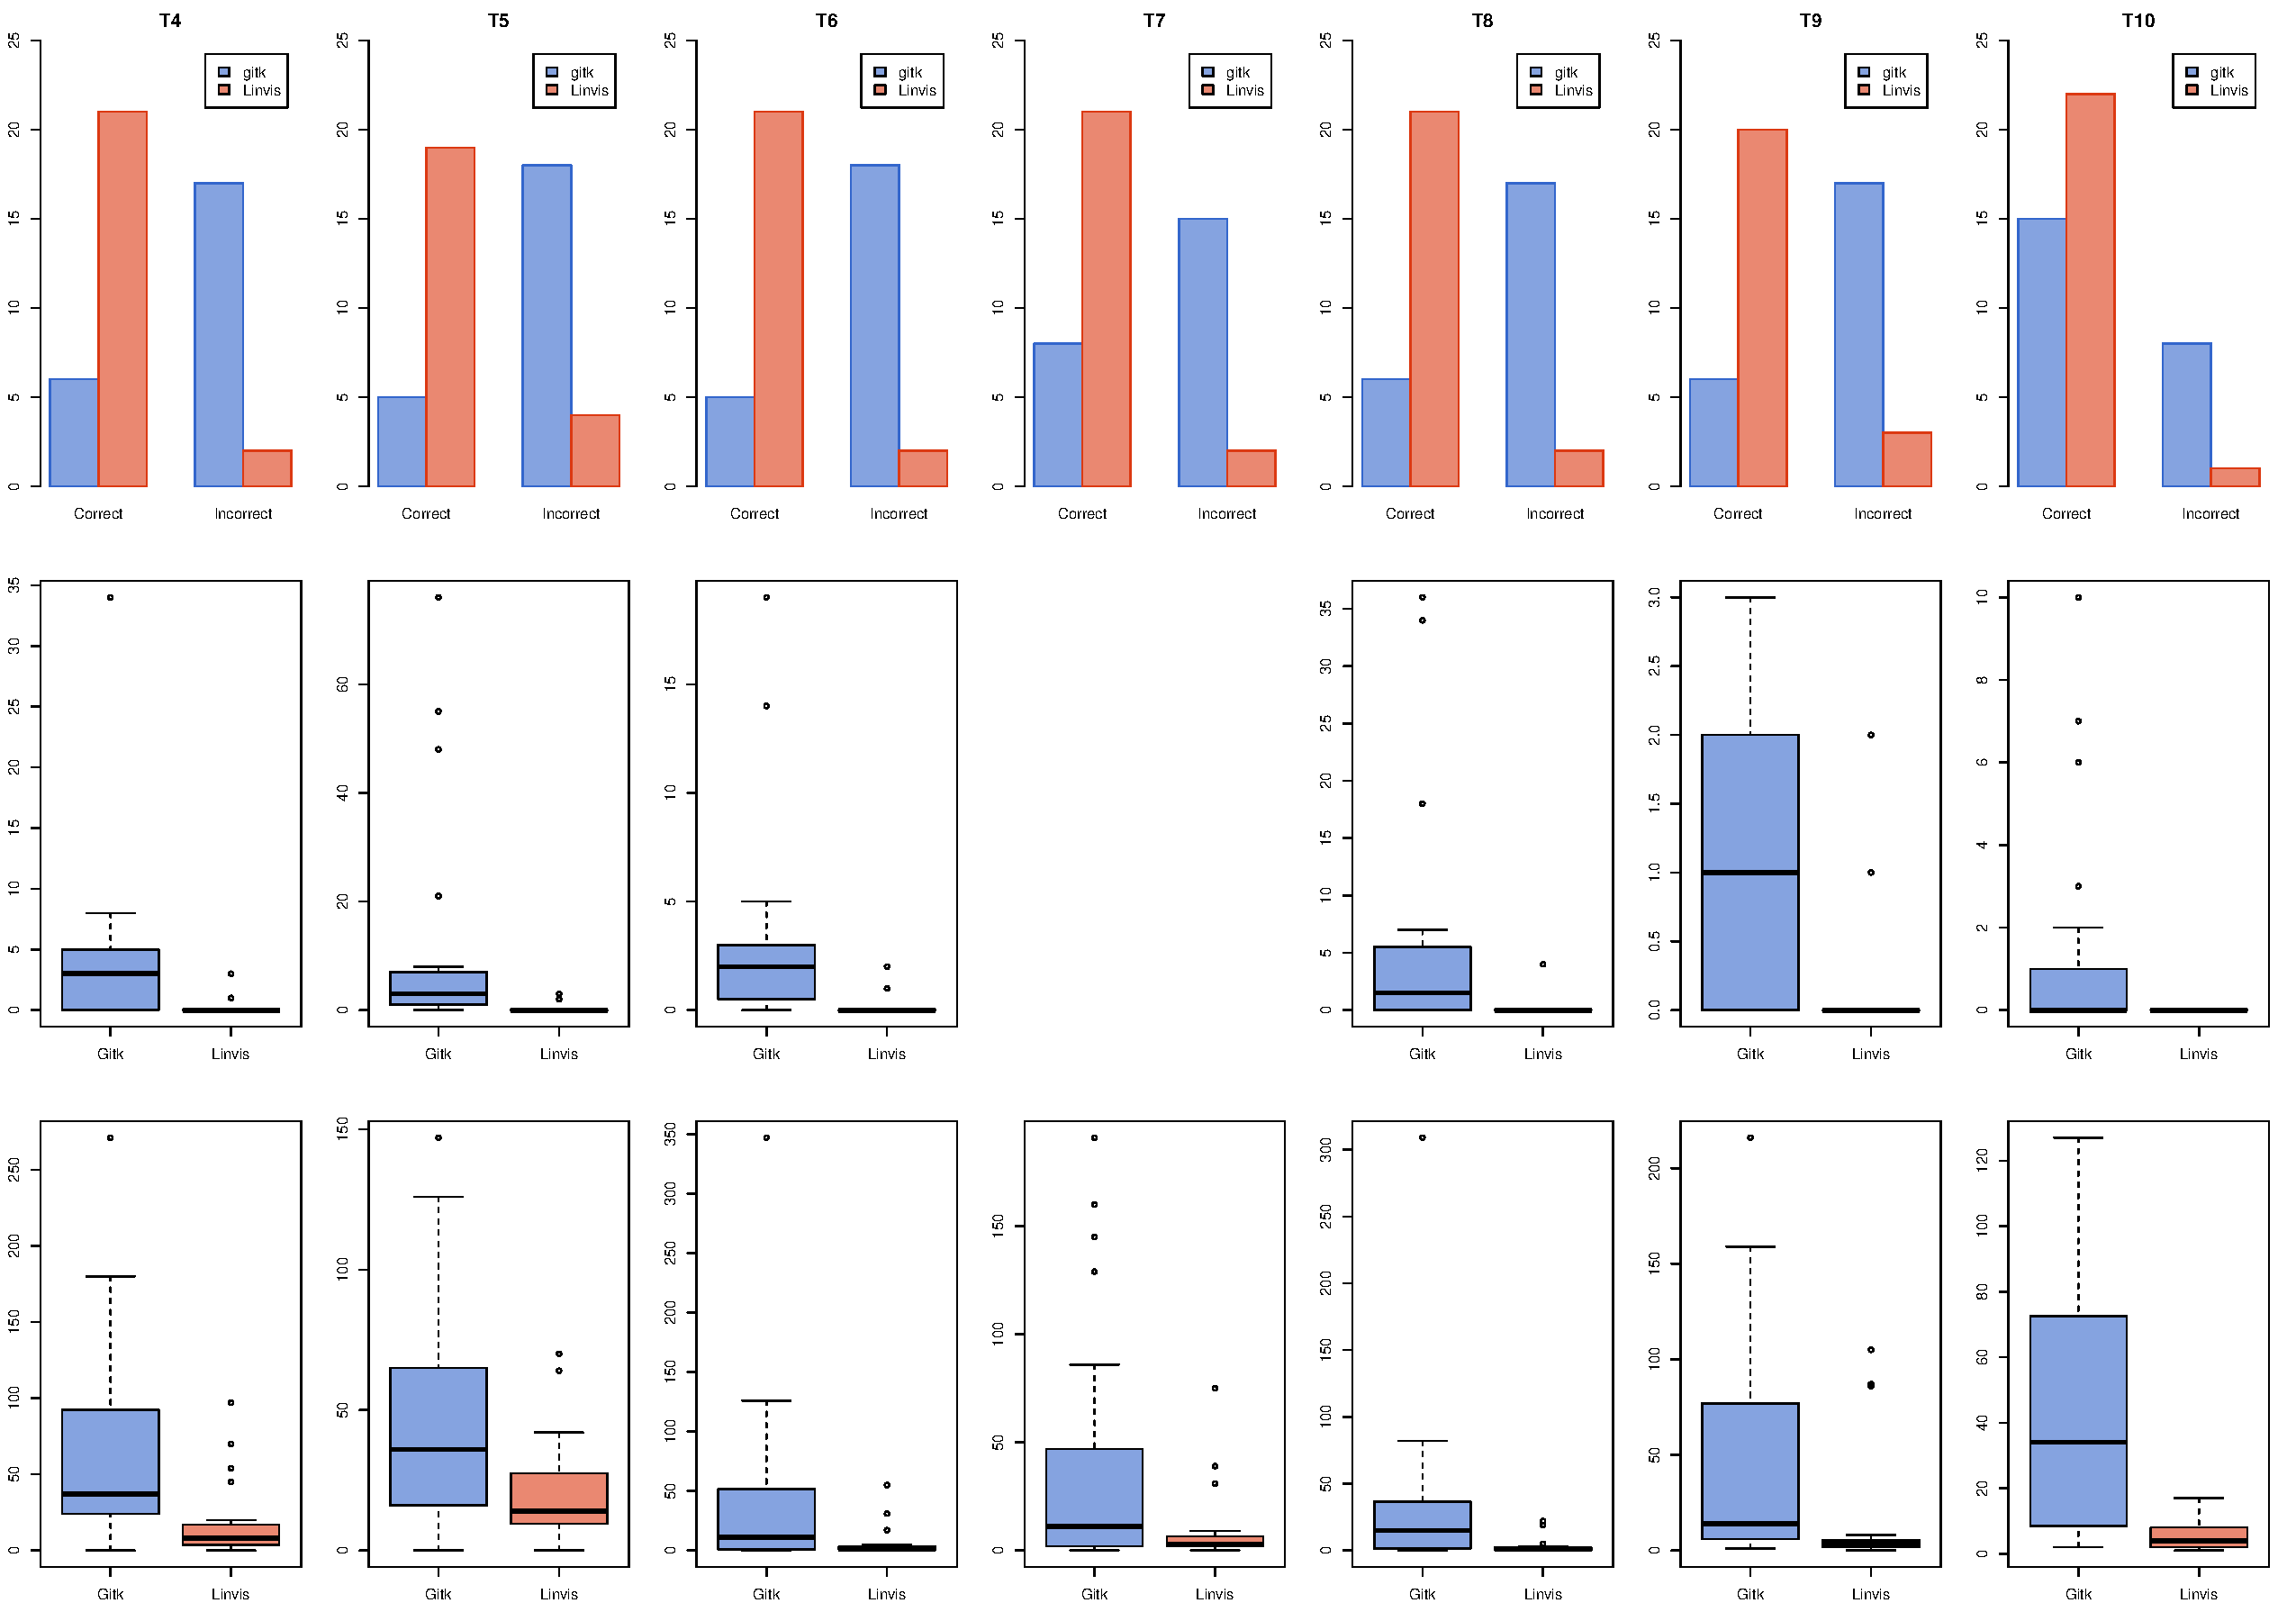
\includegraphics[width=\textwidth]{figures/userstudy/results.pdf}
  \caption{Aggregated results from the summarization tasks. The first row plots the
    correctness metric for each task. The second row plots the
    accuracy metric for each task. The third row plots the time metric
    for each task. The correctness results for T5, T9, and the timing
    results for T7 cannot be aggregated across commits, thus are
    omitted.}
  \label{fig:summarization_results}
\end{figure*}

\begin{figure*}[htpb]
  \centering

  \begin{tabular}{ m{6cm} m{6cm} }
    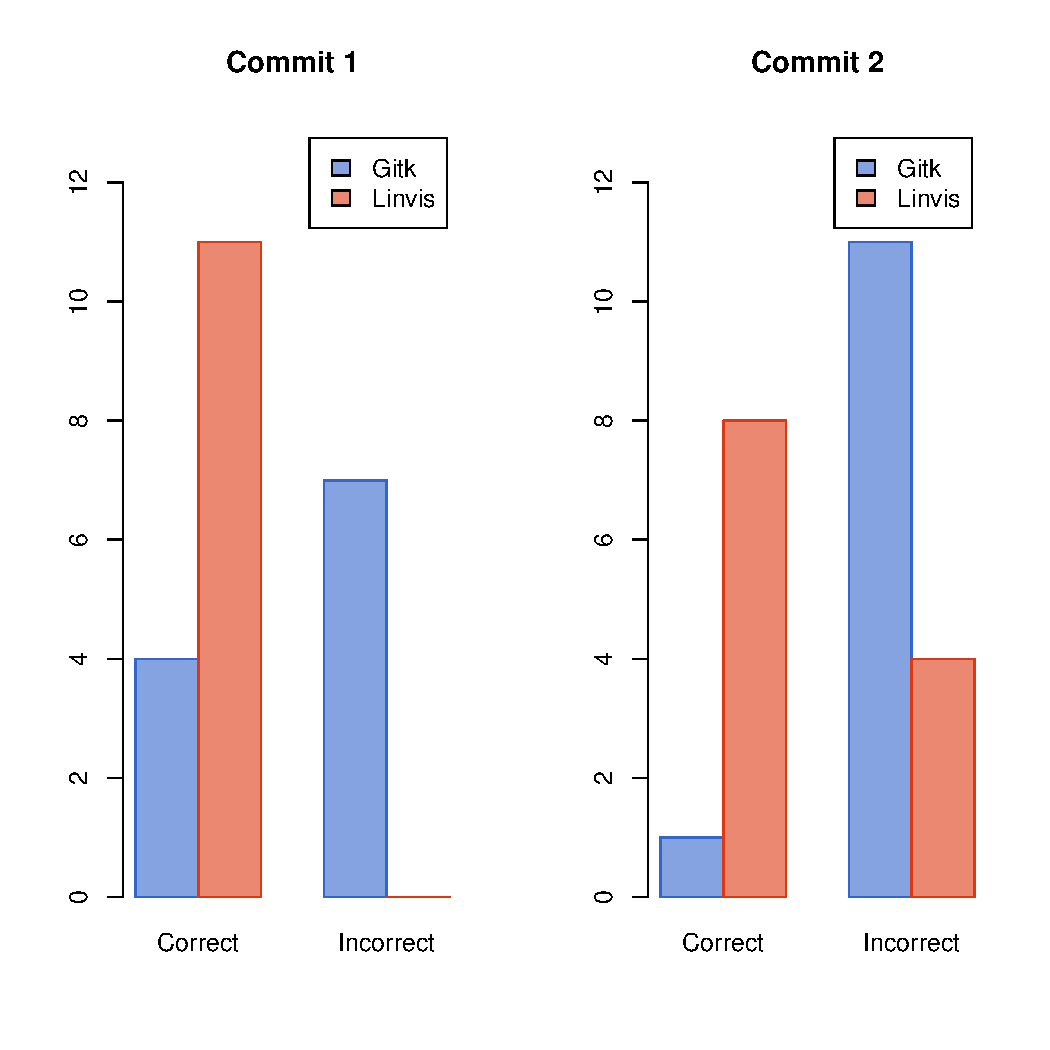
\includegraphics[width=6cm]{figures/userstudy/correctness/5.pdf} &
    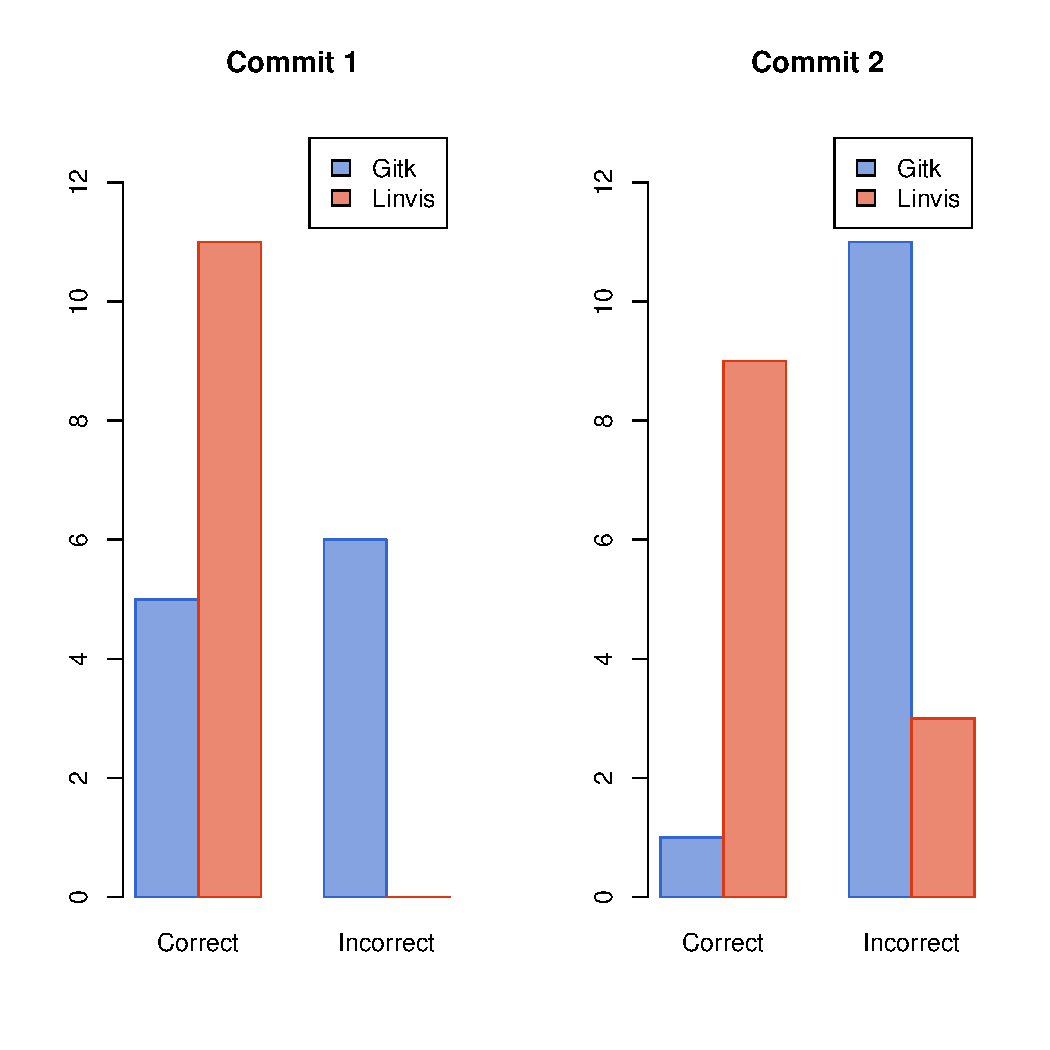
\includegraphics[width=6cm]{figures/userstudy/correctness/9.pdf}
  \end{tabular}
  \caption{Unaggregated Correctness results for T5 and T9 \evan{Split
      this? Is it clear that between Commit 2 and Commit 1 is where the
    separation of the plots is?}}
  \label{fig:correctness_t5_t9}
\end{figure*}

\begin{figure}[htpb]
  \centering
  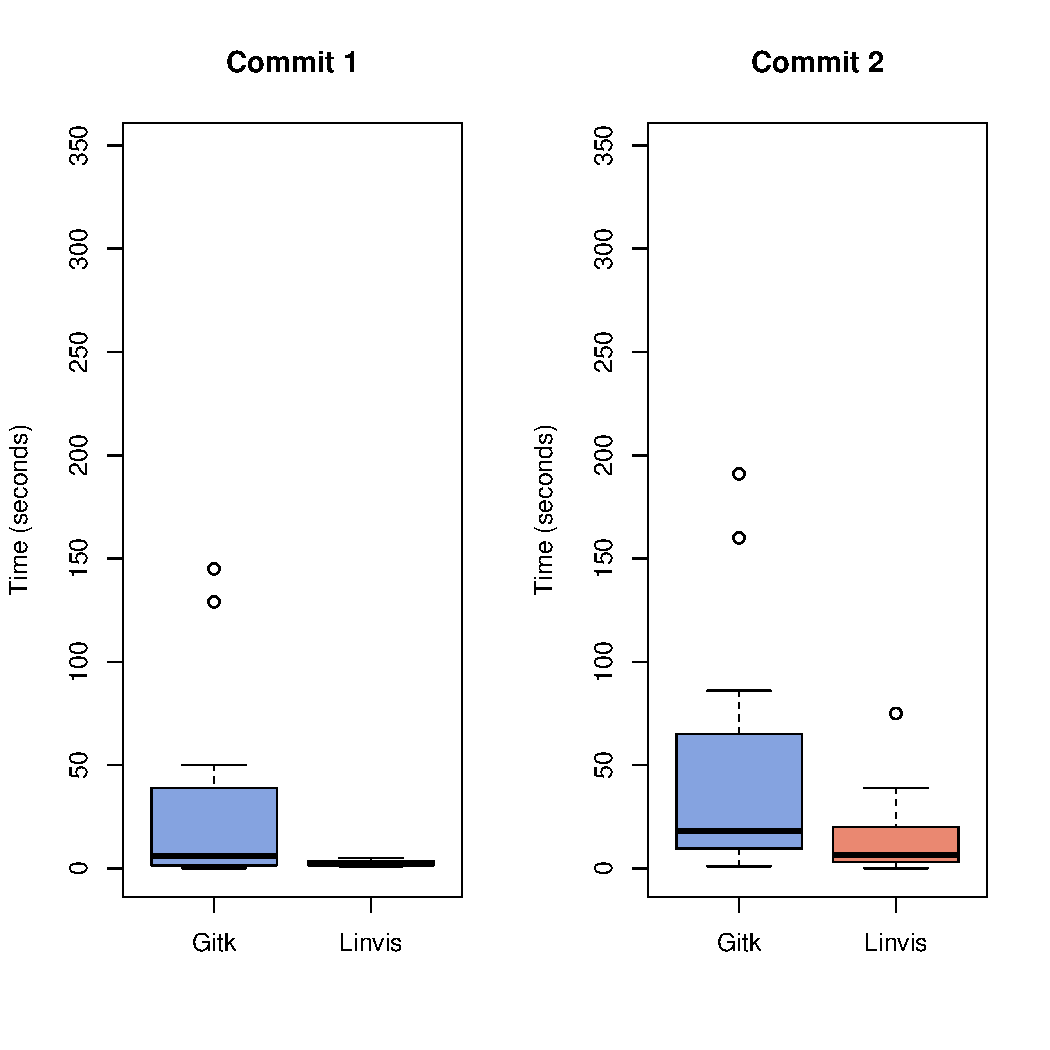
\includegraphics[width=0.8\linewidth]{figures/userstudy/time/7.pdf}
  \caption{Unaggregated Timing results for T7}
  \label{fig:timing_t7}
\end{figure}

\begin{table*}[htpb]
  \centering
  \caption{Summarized Correctness, Accuracy, and Timing results for the summarization tasks}
  \label{tab:summarization_table}
  \begin{tabular}{ccc}
    % Correctness
    \begin{tabular}{crrc}
      \toprule
      Task                  & $\chi^2$ & $p$-value  & Conclusion\\\midrule
      T4                    & 13.07    & 0.0003     & Reject $H_0$\\
      \multirow{2}{*}{T5}   & 5.14     & 0.0233     & Reject $H_0$\\
                            & 5.14     & 0.0233     & Reject $H_0$\\
      T6                    & 14.06    & 0.0002     & Reject $H_0$\\
      T7                    & 11.07    & 0.0009     & Reject $H_0$\\
      T8                    & 13.07    & 0.0003     & Reject $H_0$\\
      \multirow{2}{*}{T9}   & 4.17     & 0.0412     & Reject $H_0$\\
                            & 6.13     & 0.0133     & Reject $H_0$\\
      T10                   & 4.00     & 0.0455     & Reject $H_0$\\
      \bottomrule
    \end{tabular}
    &

    % Accuracy
    \begin{tabular}{clrc}
      \toprule
      Task & $p$-value            & Delta Est. & Conclusion\\\midrule
      T4   & $7.8 \times 10^{-5}$ & -0.61      & Reject $H_0$\\
      T5   & $7.2 \times 10^{-5}$ & -0.63      & Reject $H_0$\\
      T6   & $1.2 \times 10^{-5}$ & -0.69      & Reject $H_0$\\
      T8   & $5.8 \times 10^{-4}$ & -0.54      & Reject $H_0$\\
      T9   & $0.009$              & -0.42      & Reject $H_0$\\
      T10  & $0.002$              & -0.35      & Reject $H_0$\\
      \bottomrule
    \end{tabular}
    &
    % Timing
    \begin{tabular}{clrc}
      \toprule
      Task                 & $p$-value & Delta Est. & Conclusion\\\midrule
      T4                   & 0.0007    & -0.58      & Reject $H_0$\\
      T5                   & 0.0142    & -0.42      & Reject $H_0$\\
      T6                   & 0.0168    & -0.41      & Reject $H_0$\\
      \multirow{2}{*}{T7}  & 0.2586    & -0.29      & Do not reject $H_0$\\
                           & 0.0780    & -0.43      & Do not reject $H_0$\\
      T8                   & 0.0009    & -0.57      & Reject $H_0$\\
      T9                   & 0.0002    & -0.63      & Reject $H_0$\\
      T10                  & 0.0001    & -0.66      & Reject $H_0$\\
      \bottomrule
    \end{tabular}
  \end{tabular}
\end{table*}

Summaries for correctness, accuracy, and timing are shown in
tables~\ref{tab:summarization_table}.
The full results are as follows;

\begin{itemize}
  \item \emph{T4}: What is the series of merges involved with merging this
    commit?

    \textbf{Correctness:}
    The $\chi^2$ statistic is $13.07$ with a p-value of $0.0003$.
    $13.07 > 3.841$ and $0.0003 < 0.05$, therefore we reject the null
    hypothesis.

    \vspace{2mm}
    \begin{tabular}{cc|rr}
                            &           & \multicolumn{2}{c}{Linvis}\\
                            &           & Correct                      & Incorrect\\\hline
      \multirow{2}{*}{Gitk} & Correct   & 6                            & 0\\
                            & Incorrect & 15                           & 2\\
    \end{tabular}
    \vspace{3mm}

    \tool improves the correctness when determine the series of merges
    involved with merging a commit.

    \textbf{Accuracy:} The p-value is $7.8 \times 10^{-5}$, which is
    less than 0.05; therefore we reject the null hypothesis. The Delta
    estimate is -0.61, which indicates a large effect size. \tool
    improves accuracy when determining the series of merges involved
    with merging a commit.

    \textbf{Timing:}
    The p-value is $0.0007$, which is less than 0.05; therefore we
    reject the null hypothesis. The delta estimate is -0.58, which
    indicates a large effect size. \tool decreases the time taken to
    determine the series of merges involved with merging a commit.

    Overall, \tool is able to help users determine the series of merges
    that a commit takes more quickly and more accurately than Gitk.

  \item \emph{T5}: What other commits are merged with this commit?

    \textbf{Correctness:}
    The correctness results are split for this task. For \comA, the
    $\chi^2$ statistic is $5.14$ with a $p-value$ of $0.02334$. $5.14 >
    3.841$ and $0.02334 < 0.05$, therefore we reject the null
    hypothesis.

    \vspace{2mm}
    \begin{tabular}{cc|rr}
                             &           & \multicolumn{2}{c}{Linvis}\\
                             &           & Correct                      & Incorrect\\\hline
      \multirow{2}{*}{Gitk}  & Correct   & 4                            & 0\\
                             & Incorrect & 7                            & 0\\
    \end{tabular}
    \vspace{3mm}

    The $\chi^2$ statistic for \comB is $5.14$ with a p-value of
    $0.02334$. $4.14 > 3.841$ and $0.02334 < 0.05$, therefore we reject
    the null hypothesis.

    \vspace{2mm}
    \begin{tabular}{cc|rr}
                             &           & \multicolumn{2}{c}{Linvis}\\
                             &           & Correct                      & Incorrect\\\hline
      \multirow{2}{*}{Gitk}  & Correct   & 1                            & 0\\
                             & Incorrect & 7                            & 4\\
    \end{tabular}
    \vspace{3mm}

    While there is a difference in correctness between different-sized
    \mt{s}, \tool improves correctness of determining the other
    commits related to a commit in trees of varying sizes. The
    difference in the two commits stem from the participants that did
    not change outcomes between the tools.

    \textbf{Accuracy:}
    The p-value is $7.2 \times 10^{-5}$, which is less than 0.05;
    therefore we reject the null hypothesis. The Delta estimate is
    -0.63, which indicates a large effect size. \tool improves
    accuracy when determining other commits related to a commit.

    \textbf{Timing:}
    The p-value is $0.0142$, which is less than 0.05; therefore we
    reject the null hypothesis. The delta estimate is -0.58, which
    indicates a large effect size. \tool decreases the time taken to
    determine other commits related to a commit.

    Overall, \tool helps users determine other commits that are merged
    with another commit more quickly and more accurately.

  \item \emph{T6}: How many authors are involved in this merge?

    \textbf{Correctness:}
    The $\chi^2$ statistic is $14.06$ with a p-value of $0.0002$.
    $14.06 > 3.841$ and $0.0002 < 0.05$, therefore we reject the null
    hypothesis.

    \vspace{2mm}
    \begin{tabular}{cc|rr}
      &           & \multicolumn{2}{c}{Linvis}\\
      &           & Correct                      & Incorrect\\\hline
      \multirow{2}{*}{Gitk} & Correct   & 5                            & 0\\
      & Incorrect & 16                           & 2\\
    \end{tabular}
    \vspace{3mm}

    \tool improves correctness when determining how many authors are
    involved with a merge.

    \textbf{Accuracy:} The p-value is $1.2 \times 10^{-5}$, which is
    less than 0.05; we reject the null hypothesis. The delta estimate is
    -0.69, which indicates a large effect size. \tool improves accuracy
    when determining how many authors are involved with a merge.

    \textbf{Timing:} The p-value is 0.0168, which is less that 0.05; we
    reject the null hypothesis. The delta estimate is -0.41, which
    indicates a medium effect size. \tool decreases the time taken to
    determine the number of authors involved in a commit.

    Overall, \tool assists users with determining the number of authors
    involved in a merge more quickly and more accurately.

  \item \emph{T7}: Who contributed the most changes to this merge?

    \textbf{Correctness:}
    The $\chi^2$ statistic is $11.07$ with a p-value of $0.0009$.
    $11.07 > 3.841$ and $0.0009 < 0.05$, therefore we reject the null
    hypothesis.

    \vspace{2mm}
    \begin{tabular}{cc|rr}
      &           & \multicolumn{2}{c}{Linvis}\\
      &           & Correct                      & Incorrect\\\hline
      \multirow{2}{*}{Gitk} & Correct   & 8                            & 0\\
      & Incorrect & 13                           & 2\\
    \end{tabular}\\
    \vspace{3mm}

    \tool improves the correctness of participants when determining the
    author that contributed the most changes to a merge.

    \textbf{Timing:} The null hypothesis is not rejected in the case of
    \comA, but is rejected in the case of \comB. This indicates that
    \tool is able to help users determine who made the most
    contributions to a merge in a large tree but not in a small tree.

    Overall, \tool improves the correctness for trees of various sizes,
    but only has an effect on the length of time taken when the tree is
    large.

  \item \emph{T8}: How many files were modified in this merge?

    \textbf{Correctness:}
    The $\chi^2$ statistic is $13.07$ with a p-value of $0.0003$.
    $13.07 > 3.841$ and $0.0003 < 0.05$, therefore we reject the null
    hypothesis.

    \vspace{2mm}
    \begin{tabular}{cc|rr}
      &           & \multicolumn{2}{c}{Linvis}\\
      &           & Correct                      & Incorrect\\\hline
      \multirow{2}{*}{Gitk} & Correct   & 6                            & 0\\
      & Incorrect & 15                           & 2\\
    \end{tabular}\\
    \vspace{3mm}

    \tool improves the correctness of users when determining the number
    of files that were modified in a merge.

    \textbf{Accuracy:} The p-value is $5.8 \times 10^{-4}$, which is
    less than 0.05; we reject the null hypothesis. The delta estimate is
    -0.54, indicating a large effect size. \tool improves accuracy when
    determining how many files were modified at a merge.

    \textbf{Timing:} The p-value is 0.0009, which is less than 0.05; we
    reject the null hypothesis. The delta estimate is -0.57, indicating
    a large effect size. \tool decreases the time taken to determine the
    number files modified in a merge.

    Overall, \tool assists users to determine the number of files
    modified in a merge more quickly and accurately.

  \item \emph{T9}: Which file(s) had the most changes in this merge?

    \textbf{Correctness:}
    The correctness results are split for this task. For \comA, the
    $\chi^2$ statistic is $4.17$ with a p-value of $0.0412$. $4.17 >
    3.841$ and $0.0412 < 0.05$, therefore we reject the null hypothesis.

    \vspace{2mm}
    \begin{tabular}{cc|rr}
                             &           & \multicolumn{2}{c}{Linvis}\\
                             &           & Correct                      & Incorrect\\\hline
      \multirow{2}{*}{Gitk}  & Correct   & 5                            & 0\\
                             & Incorrect & 6                            & 0\\
    \end{tabular}
    \vspace{3mm}

    The $\chi^2$ statistic for \comB is $6.125$ with a p-value of
    $0.0133$. $6.125 > 3.841$ and $0.0133 < 0.05$, therefore we reject
    the null hypothesis.

    \vspace{2mm}
    \begin{tabular}{cc|rr}
                             &           & \multicolumn{2}{c}{Linvis}\\
                             &           & Correct                      & Incorrect\\\hline
      \multirow{2}{*}{Gitk}  & Correct   & 1                            & 0\\
                             & Incorrect & 8                            & 3\\
    \end{tabular}
    \vspace{3mm}

    While there is a different in correctness between different-sized
    \mt{s}, \tool improves the correctness when determining which files
    had the most changes in trees of varying sizes. The difference in
    the two commits stem from the participants that did not change
    outcomes between tools.

    \textbf{Accuracy:} The p-value is $0.009$, which is less than
    $0.05$; we reject the null hypothesis. The delta estimate is -0.42,
    indicating a medium effect size. \tool improves accuracy when
    determining which file had the most changes.

    \textbf{Timing:} We reject the null hypothesis; the delta estimate
    is -0.63, indicating a large effect size. \tool decreases the time
    taken to determine which file had the most changes.

    Overall, \tool is able to assist users determine which file had the
    most changes more quickly and accurately.

  \item \emph{T10}: Which modules does this \mt involve?

    \textbf{Correctness:}
    The $\chi^2$ statistic is $4$ with a p-value of $0.0455$.
    $4 > 3.841$ and $0.0455 < 0.05$, therefore we reject the null
    hypothesis. The p-value is very close to the $\alpha$ value in this
    case, so the conclusion is not as well defined.

    \vspace{2mm}
    \begin{tabular}{cc|rr}
      &           & \multicolumn{2}{c}{Linvis}\\
      &           & Correct                      & Incorrect\\\hline
      \multirow{2}{*}{Gitk}   & Correct   & 14                           & 1\\
      & Incorrect & 8                            & 0\\
    \end{tabular}
    \vspace{3mm}

    \tool improves correctness when determining the modules involved at
    a merge.

    \textbf{Accuracy:} The null hypothesis is rejected; the delta
    estimate is -0.35, indicating a medium effect size. \tool improves
    accuracy when determining which modules are involved with a merge.

    \textbf{Timing:} The null hypothesis is rejected; the delta estimate
    is -0.66, indicating a large effect size. \tool decreases the time
    taken to determine the modules involved with a merge.

    Overall, \tool assists users determine which modules are involved
    with a merge more quickly and accurately.

\end{itemize}

\tool is able to assist users with summarizing various aspects of a
merge more quickly and accurately than Gitk. In two tasks, T5 and T9,
correctness was affected by the size of a tree, but in both trees, \tool
was able to provide a statistically significant improvement to the
correctness. Only in one task, T7, was timing affected by the size of a
tree; \tool did not significantly improve the time taken to answer T7 on
the smaller tree, but did improve the time taken on the larger tree.

\subsubsection{User Opinions}
\label{sub:user_opinions}

Among the 12 participants, there was nearly unanimous agreement that for
conceptual understanding and summarization tasks; \tool was easier to
work with than Gitk. The participants cited the ability to abstract
information about the merge from the clean summarization tables and
simple visualizations. Three participants suggested that someone with a
professional understanding of Gitk and the git command-line may be to
extract a conceptual understanding from the DAG visualization and
perform the summarization tasks. One of these three participants said
that they would prefer to have both tools available, as they are able to
complement each other.

%%% Local Variables:
%%% mode: latex
%%% TeX-master: "lineval.tex"
%%% End:


\section{Discussion}
\label{sec:discussion}

% vim:set et sw=2 ts=4 tw=72:
% Jun 24, 2017

\section{Discussion}
\label{sec:discussion}

The results show conclusive results; the DAG visualization \dmg{provided by gitk...} is unable to \dmg{this is a very
  long sentence that does not read very well}
adequately provide users with an explanation of the changes being made
in the repository, the DAG visualization is not easily understood, and
is unable to provide summarizations of the changes being made at a
merge. Meanwhile, the \mt visualization \dmg{of linvis...} is better able to provide an
explanation of how a commit is integrated, along with better
summarization. In this section, we discuss some observations, threats to
the validity, and comments made by the participants during the study
followed by discussion about modifications to the original algorithm to
help generalize it for more repositories, concluded with future work.

% TODO: Future work?

\subsection{Observations}
\label{sub:observations}

% \dmg{I think you mean challenge using gitk, right? so be explicit}

During the course of the study, we noticed an issue that was consistent
among the participants when using Gitk; \dmg{wrong use of semicolon} the most difficult challenge was
identifying the master branch of the repository. Many participants would
identify the tag as being the ``master branch'', but a tag is not a
branch (it simply points to a given commit). The visualization of the DAG does not provide any notion of
which branch being shown is the master branch. The default assumption is
that the first branch on the left is the master branch, but this is not
always correct. Furthermore, the visualization in Gitk is not
consistent, the ordering of the branches changes between runs, so
identifying the branch once will not guarantee that it will be
identifiable after restarting Gitk.\dmg{i didn't know the ordering is non-deterministic, are you sure? make sure you are
sure, sure? :)}

If users were able to easily identify the master branch using the
visualizations of the DAG, the results of the study would likely be very
different\dmg{be explicit eg.: that there was very little difference, if any, between the use of both tools}. This would
certainly be the case for the single-commit tree; \dmg{another wrong use, i want you to read the description of colon vs
semicolon and scan the paper for them to make sure they are used correctly}
it is trivial to summarize information about a single item, but
identifying that there was only a single commit in the tree was
non-trivial. This information is important because many trees contain a
single commit, and the structure of these trees is identical to the
structure of flat trees. Flat trees are the most common branching
structure in the repository, with the root being the parent to all of
the other nodes in the tree; to improve summarization and comprehension
of these trees, it would likely by sufficient to indicate the master
branch in the DAG visualization.

While, in general, the participants of the study preferred using \tool
to Gitk, there were some noticeable usability issues in \tool. The most
prominent issue being the navigation within the tree visualizations. The
participants expected that the tabs would update when they clicked on a
node in the tree, instead of having to click the link to the commit
after clicking the node. This was true in both the \rt tree and the Pack
tree. The second major usability issue was the inconsistency between the
list tree and the other tree visualizations. The list tree is rooted at
the repository event that the user is current looking at, while the
other tree visualizations show the entire tree, and use bright orange to
highlight the current node.


\subsection{Comments From a Release Manager}
\label{sub:comments_from_a_release_manager}

One participant in the study worked as a release manager for more than
three years, working with both SVN and CVS repositories, but had little
experience with git. This subsection contains improvements made by this
participant during the study and afterward.\dmg{he made improvements? to what? Isn't this section about his views of
  what is needed?}

Contributors making merges need to understand more than just what merges
a commit was collected into before reaching the repository of the
contributor. It is also important to understand order that the related
commits were made, as the order tells the story of what the developer
was thinking as they were writing the changes. The current \mt model
does not order the commits, simply placing them randomly. \dmg{this surprised me. we order the commits in the tree, you
  know which is before which, so this is more an issue of you not displaying the data than we not having it} This is the
primary reason behind this participant's request to use both \dmg{tools}
simultaneously. \tool is able to help with the aggregation of the
information, and provide a better understanding of the next merge
involved in integrating this commit, but the DAG visualization in Gitk
provides the full story of the commit instead of hiding it behind a
layer of abstraction.

The comments from this participant were very insightful, and will assist
in improving the model in the future.

\subsection{Threats to Validity}
\label{sub:threats}

\textbf{Internal Threats:}

The repository contains many commits, of which we only chose two. The
commits chosen were randomly selected to be representative of those in
the repository. Additional commits could be added, but this would
include additional time costs during the study.

The answers provided by the participants to earlier tasks were not
taken into account for determining the accuracy\dmg{accuracy of what? the stattement is not clear to me. Oh, i think you
mean, if they get an answer wrong it might impact the results of some following tasks; you can be more precise in the description}. If the participant was
unable to determine the correct commits for the tree within the
conceptual task group, the summarization results would be recorded as
wrong, even if the summarization they provided was correct for the set
of commits selected to be part of the tree. A further study could be
done where the correct answer was provided to the participant after each
task so that errors would not propagate between tasks.

To mitigate the effects of order-bias, the order the tasks were
performed, the tools were used, the commits were studied was shuffled
between participants. A single participant is affected by the effect,
but this should be mitigated by the results from other participants.

We were only able to work with 12 participants. We apply various
statistical tests to ensure that our findings are statistically significant.

\textbf{External Threats:}

While git includes Gitk and git log provides a visualization of the DAG
with \verb|git log --graph|, many of the participants in our study were
unfamiliar with the DAG visualizations shown by these tools. Other tools
may provide better summarizations and visualizations, but we are unaware
of any. We investigated the gui tools for Linux on the git
website\footnote{\url{https://git-scm.com/download/gui/linux}}, but none
of the tools, with the exception of Gitk and git log, were able to
produce a visualization of the DAG for the Linux repository.
Investigating the tools more deeply, it appears that GitKraken is the
most popularly cited git client. The visualization provided by GitKraken
was centered around the same DAG metaphor used by git log. GitKraken was
unable to produce a visualization for the Linux repository on our
system. Inspecting these tools on smaller repositories show that the
visualizations of the DAG were very similar to the visualization in
Gitk.

\dmg{add a couple of sentences on the fact that these were students, some with industrial experience. People who are
  professinals might do better}

% A possible

% reason for this may be that unless a repository reaches a sufficient
% complexity, both in branching and number of commits, these tools are
% unnecessary for the normal operation of git. Furthermore, fear of the
% complexity caused by branching may cause personal and academic
% repositories to have relatively simple structures. While they were
% unfamiliar with the DAG structure, these users were also unfamiliar with
% the \mt model, and were still able to better understand and summarize
% the repository using \tool.

\dmg{the following should be a section on its own, because it is no longer part of the study, also
use a better title: generalization of the creation of the merge-tree?}

\subsection{Generalization}
\label{sub:generalization}

Seeing that the visualizations of the \mt model are able to assist users
with understanding how commits are integrated, we continue by looking at
ways of improving the algorithm for faster operations, and making the
conversion from DAG to \mt feasible over the internet.

The problem of identifying the master branch is the most difficult, and is
not possible without heuristic approaches. The master branch can be
confounded by \foxtrot merges, which change the order of the
parents in the parent list of a merge. Other than the ordering of the
parent list, git has no other way to determine which commits are on the
master branch of the repository. For the purpose of this discussion, we
will assume that we can rely on the order of the parent list to be
correct, and that \foxtrot{s} do not occur. Furthermore, merge
information is lost in the event of fast-forward merges, which collapse
the branch into the current branch.

\begin{algorithm}
  \caption{Computing the generalized Merge Tree}
  \label{alg:generalized}
  \begin{algorithmic}[1]
    \Function{Phase 1}{initial commit $root$} : updated tree
    \State $openBranches \gets 0$
    \State $Q \gets root$
    \Do
    \State $cur \gets Q.dequeue$
    \State $parents \gets cur.parents$
    \State $openBranches \gets openBranches + parents.length - 1$
    \For{$index, parent \in parents$}
    \If{$parent.depth$ is $undefined$}
    \State $parent.depth \gets cur.depth + index$
    \ElsIf {$cur.depth > parent.depth$}
    \State $openBranches \gets openBranches - 1$
    \ElsIf {$cur.depth < parent.depth$}
    \State $openBranches \gets openBranches - 1$
    \State $parent.depth \gets cur.depth$
    \EndIf
    \State $parent.children \gets cur$
    \If{$parent$ has not been visited}
    \State $Q \gets parent$
    \State $parent.visited \gets True$
    \EndIf
    \EndFor
    \doWhile{$Q$ not empty and $openBranches \ne 0$ }
    \EndFunction

    \Function{Phase 2}{initial commit $root$} : Merge tree
    \State $tree.root \gets root$
    \State $Q$ // Empty Queue

    \State $parents \gets root.parents$
    \State $parents \gets tail\ parents$
    \For {$parent \in parents$}
    \State $realParent \gets min(\forall child \in parent.children,\ parent.depth >= child.depth)$
    \If {$realParent$ is $root$}
    \State $root.children \gets parent$
    \State $parent.parent \gets root$
    \State $Q \gets parent$
    \EndIf
    \EndFor

    \While{$Q$ not empty}
    \State $cur \gets Q.dequeue$
    \State $parents \gets cur.parents$
    \For{$parent \in parents$}
    \State $realParent \gets min(\forall child \in parent.children,\ parent.depth >= child.depth)$
    \If {$realParent$ is $cur$}
    \State $cur.children \gets parent$
    \State $parent.parent \gets cur$
    \State $Q \gets parent$
    \EndIf

    \EndFor
    \EndWhile

    \EndFunction
  \end{algorithmic}
\end{algorithm}

The primary difference between the original algorithm and the
generalization is the main data structure. Algorithm~\ref{fig:alg}
is centered around the use of the stack, making it akin to a depth-first
traversal of the DAG with dynamic programming. The generalization in
Algorithm~\ref{alg:generalized} is based on the queue, making it akin to
the breadth-first traversal of the DAG.\@ While the final results of the
two traversals should not be different, the runtime properties are
different.

We will begin with a simplified description of the original algorithm.
The algorithm starts at the reference to the master branch. We will use
the term master branch loosely here, meaning any branch that has been
labeled in some way as being the main branch, this branch may have a
different name, but standard naming conventions call it the master
branch. Starting from the master branch label, we traverse the entire
master branch to the initial commit, recording the commit hash of every
repository event encountered.

The second phase iterates over every repository event, computing the
shortest distance to the master branch. For this reason, the entire
repository must be available to the algorithm. This is a dynamic
programming solution, centered around the call stack. The next node on
the shortest path to the master branch will become the parent of this
node in the tree.

\dmg{you don't generalize an alg into a tool; you implement the algorithm in a tool}
If this algorithm is to be generalized into a dynamic, web-based, tool,
it may not be feasible to download every every repository event in the
repository in a reasonable period of time. We instead look toward a
breadth-first approach at limiting the number of repository events that
must be downloaded.

Focusing on the generalized algorithm (Algorithm~\ref{alg:generalized}),
the algorithm is broken into two phases. The first phase is where the
improvements take place. The first phase has three main goals; the first
is to track the master branch; the second goal labels the depth of each
repository event that is traverses, or how many merges the event is from
being merged; the third goal is to record the children of each
repository event. The first phase also begins the process of reversing
the DAG, by providing the candidate events that could possibly be the
real parent to this node. The first phase can terminate early, if it
reaches a point where all branches that it is following terminate. The
$openBranches$ metric on line 7 indicates how many branches are
currently being traversed. In line 11 through 15, we decrement the
$openBranches$, as this is the point where a branch occurs. The second
branch closing clause is necessary to handle the case when the depth was
incorrectly assigned, which can occur if there are more events on the
current branch than on the side branch.

\begin{table}[htpb]
  \centering
  \caption{Example traversal of the example DAG in
    Figure~\ref{fig:repoDAG} starting at merge 11.}
  \label{tab:ex_traversal}
  \begin{tabular}{cccc|cc}
    \toprule
    Current & Parents & Open Branches & Q       & Visited & Children\\\midrule
    -       & -       & 0             & 11      & 11:0    & \\
    11      & 4,9     & 1             & 4,9     & 4:0     & 11, 5\\
    4       & 1       & 1             & 9,1     & 9:1     & 11\\
    9       & 7,6,8   & 3             & 1,7,6,8 & 7:1     & 9, 8\\
    1       &         & 3             & 7,6,8   & 6:2     & 9\\
    7       & 5       & 3             & 6,8,5   & 8:3     & 9\\
    6       & 5       & 2             & 8,5     & 5:1     & 7, 6\\
    8       & 7       & 1             & 5       & 2:1     & 5, 3\\
    5       & 4,2,3   & 2             & 2,3     & 3:2     & 5\\
    2       & 1       & 1             & 3       &         & \\
    3       & 2       & 0             &         &         & \\
    \bottomrule
  \end{tabular}
\end{table}

In Table~\ref{tab:ex_traversal}, we follow the algorithm starting at
merge 11 from the example in Figure~\ref{fig:repoDAG}, recording the
current node, the parents of the current node, the open branches, and
the queue structure after updating. The visited column is not dependant
on the current step, but keeps track of the nodes that have been
visited, the depth, and the children of the corresponding node. When we
reverse the DAG, the children in this table will become the candidates
for being the parent of the corresponding node. For example, the parent
of node 7 may be resolved to either node 9 or node 8. In this case, the
shortest path to the master branch is through node 9.

The terminology surrounding the parent/child relationship gets very
confusing at the change between phase one and two because this is where
the roles switch. In phase 1, we are working with the DAG; in phase 2,
we are working with a structure that is neither a tree nor a DAG, but
can only be described as a directed graph.

The goal of the second phase is to resolve the tree from the directed
graph. We will refer to parents in the same sense as we would refer to
them in the tree form of the repository for the remainder of this
section. We have gathered the depths and possible parents (line 17), but
we need to remove the extra parents. Extra parents are culled in line 42
of the algorithm. Of the possible parents, we take the parent that is
closest to the root, but not beyond. This forces the real parent to
either be deeper in the tree, or on the same branch as the current node.
Line 30 to 37 are for bootstrapping the queue, ensuring that we are not
starting on an empty queue and is nearly identical to lines 41 to 48.

The construction of the tree becomes trivial now that we are able to
determine the parents and children for each node. Lines 44 and 45
perform this construction, adding the DAG parent to the tree children of the
current node, and the DAG parent's parent becomes the current node,
which was the DAG parent's child. We continue following the path until
we hit the root node, merging the commit into the master branch.

This algorithm relies heavily on the order of parents in the parent
list, but is able to trim the number of nodes that must be downloaded.
Furthermore, the resulting tree is able to show the order of commits,
telling the story of how a developer was working, before the set of
commits was merged. We developed a small Bitbucket plugin to test the
design and determine whether it was capable of producing \mt{s},
shown in Figure~\ref{fig:b_plugin}.

\begin{figure}[htpb]
  \centering
  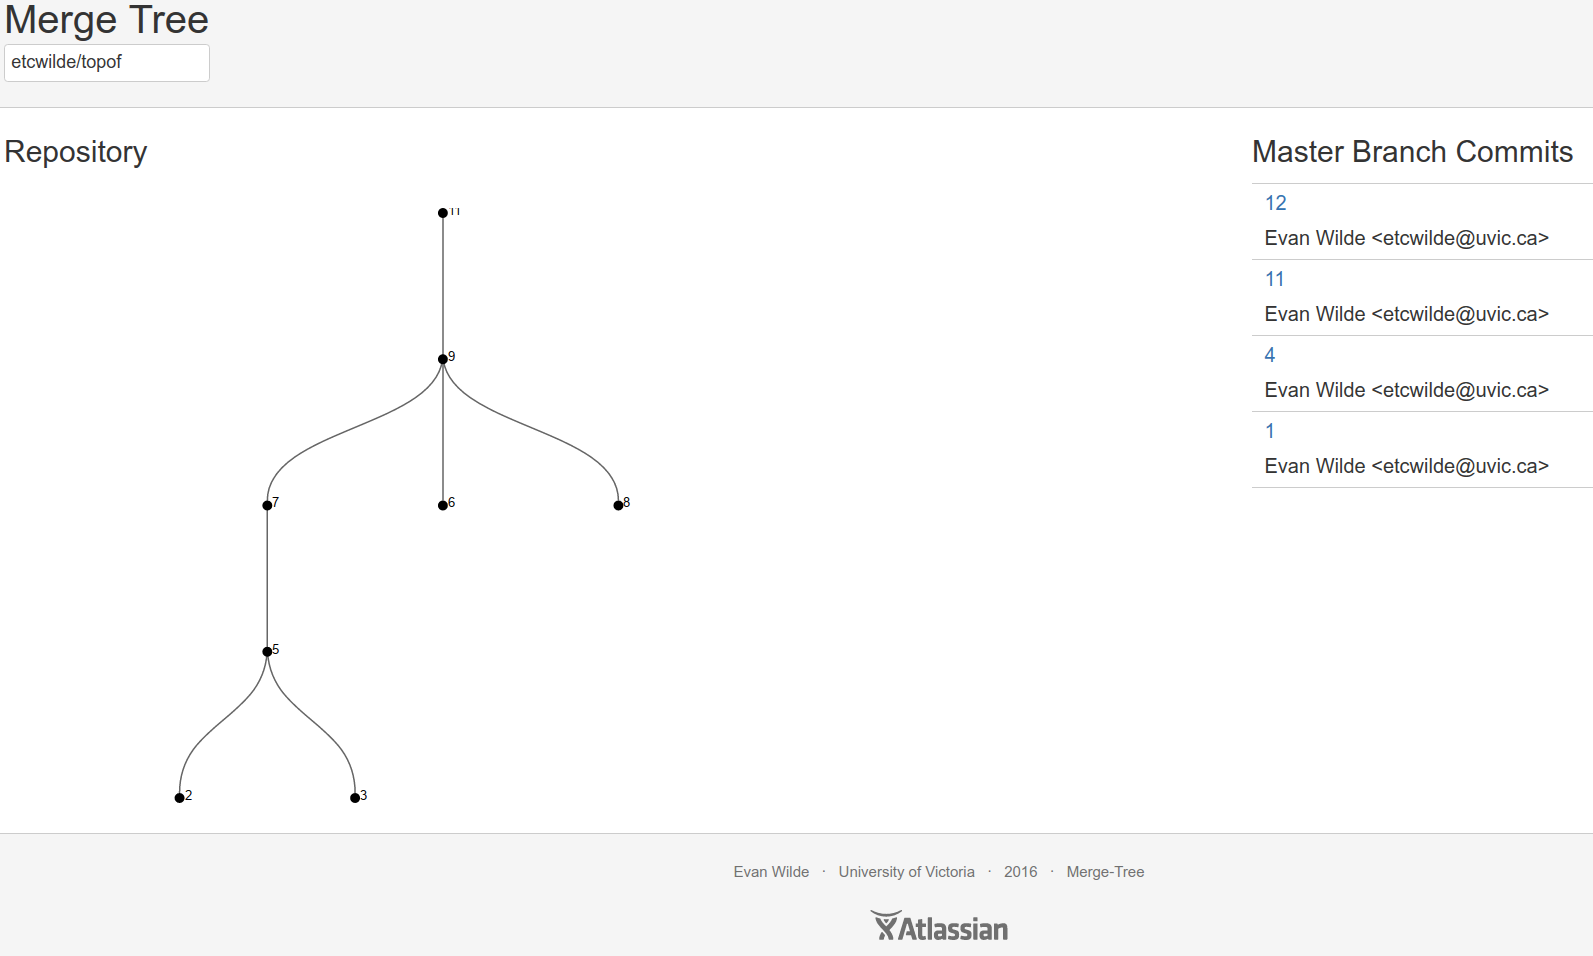
\includegraphics[width=\linewidth]{figures/plugin.png}
  \caption{Screen shot of the Bitbucket plugin showing the online tree
    computation of the repository shown in~\ref{fig:repoDAG}.}
  \label{fig:b_plugin}
\end{figure}


%%% Local Variables:
%%% mode: latex
%%% TeX-master: "lineval.tex"
%%% End:


\section{Conclusion}
\label{sec:conclusion}

\section{Conclusion}
\label{sec:conclusion}

\dmg{in this paper we describe, not develop}

In this paper, we develop a tree-based model, \mt, designed to provide git
users with a better explanation of the events occurring in a git
repository. The \mt model is rooted at the merge into the master branch
of a repository, where the leaves are the individual commits.

We implement a tool, \tool, using the \mt model, which allows a user to
filter the commits with a simple search interface. Once the user finds \dmg{user => they or he/she or users => they, tense issue?}
the commit that they are interested in, they are provided simple
aggregated tables showing the files that were modified, the authors that
made the modifications, among other information. \dmg{they is very ambiguous: are we talking authors, users, tables,
  files? be precise}
They are also provided
with three visualizations, a list tree, a pack tree, and a
Reingold-Tilford tree view. The list tree enables easy searching for
textual features, while the pack tree is good for visualizing the
structure of large \mt{s}, and the Reingold-Tilford tree is better
at visualizing the structure of small \mt{s}.

\dmg{not necessary: useful, and not only the model, but the implementation}
To ensure that our model is necessary, we evaluate the ability of users
to perform simple conceptual tasks \dmg{using linvis and comparing it with ... be precise}
, finding how a commit was merged into
the master branch of the Linux repository, and determining other commits
that were merged with the given merge. Finding that the participants in
our study were unable to perform this task \dmg{using gitk?, be precise, but you didn't ask them to compare based on
  their unability to perform the task, they were ask to do it nonetheless}, we compared the ability of
the participants to summarize key pieces of information aggregated in
these groups of commits. We asked for information about what files were
modified, the authors making the changes, among other tasks\dmg{among other tasks? tasks are T1...Tn. Don't overload
  uses of a word}. Finally, we
asked the participants about their preference in tools, and which
aspects of each they preferred. We found that the participants in our
study were able to identify the correct answer more quickly and
accuractly using the \mt visualization than they were able to with
visualizations of the DAG.

Given that visualization of the model provides users with a better
understanding of events in the repository, we describe some issues with
identifying the master branch of the repository and a more generalized
approach to constructing \mt{s}. We implement \dmg{this should be past tense} the generalized approach
as a Bitbucket plugin to verify that it is able to quickly produce
results online, unlike in the implementation of \tool.\dmg{the most important aspect is nto that it can quickly produce
  results, but that it can be applied to any repo in bitbucket}

Participants in our study found them \dmg{who/what is them?} to be more enjoyable for
summarization tasks than visualizations of the DAG.\@ While there are
some issues \dmg{with what tool? linvis?, \mt should be in the first phrase, not the ending phrase} with identifying the master branch in a robust manner, \mt
visualizations are an effective means of providing a clear conceptual
understanding and simple summarization of the events being merged into a
the master branch of a repository.


%%% Local Variables:
%%% mode: latex
%%% TeX-master: "lineval.tex"
%%% End:


\balance

% \nocite{*}

\bibliographystyle{IEEEtran}
\bibliography{references}

\end{document}

%%% Local Variables:
%%% mode: latex
%%% TeX-master: t
%%% End:
